\documentclass[13pt,a4paper]{extreport}
\usepackage[utf8]{inputenc}
\usepackage[T5]{fontenc} % Hỗ trợ tiếng Việt
\usepackage[vietnamese]{babel}
\usepackage{mathptmx} % Font Times New Roman
\usepackage{graphicx}
\usepackage{amsmath}
\usepackage{hyperref}
\usepackage{geometry}
% Căn lề: Trái 3cm (để đóng gáy), Phải 2cm, Trên 2cm, Dưới 2cm cho toàn bộ các trang
\geometry{a4paper, left=3cm, right=2cm, top=2cm, bottom=2cm}

\usepackage{setspace}
\setstretch{1.2} % Line spacing Multiply at 1.2

\setlength{\parskip}{6pt} % Spacing After 6pt
\setlength{\parindent}{1cm} % First line indent 1cm

\usepackage{eso-pic}
\usepackage{tikz}
\usepackage{fancyhdr}
\usepackage{titlesec}

% Định dạng tiêu đề chương có đánh số: CHƯƠNG I: TÊN CHƯƠNG
\titleformat{\chapter}[block]
  {\normalfont\huge\bfseries}
  {\chaptertitlename\ \thechapter:}
  {0.5em}
  {\MakeUppercase}

% Định dạng tiêu đề chương không đánh số (Mở đầu, Lời cảm ơn...)
\titleformat{name=\chapter,numberless}[block]
  {\normalfont\huge\bfseries\centering}
  {}
  {0pt}
  {\MakeUppercase}

% Đổi tên các mục mặc định sang tiếng Việt và in hoa
\addto\captionsvietnamese{%
  \renewcommand{\chaptername}{CHƯƠNG}%
  \renewcommand{\contentsname}{MỤC LỤC}%
  \renewcommand{\listfigurename}{MỤC LỤC HÌNH ẢNH}%
}

% Đánh số chương bằng số La Mã I, II, III...
\renewcommand{\thechapter}{\Roman{chapter}}
% Đánh số mục (section) sử dụng số Ả Rập 1.1, 1.1.1...
\renewcommand{\thesection}{\arabic{chapter}.\arabic{section}}
\renewcommand{\thesubsection}{\arabic{chapter}.\arabic{section}.\arabic{subsection}}

\begin{document}

% ------------------- PHẦN TRƯỚC (KHÔNG ĐÁNH SỐ TRANG) -------------------
\pagestyle{empty}
\fancypagestyle{plain}{ % Ghi đè trang đầu của chương để không có số trang
  \fancyhf{}
  \renewcommand{\headrulewidth}{0pt}
  \renewcommand{\footrulewidth}{0pt}
}

% Trang bìa

\begin{titlepage}
    \AddToShipoutPictureBG*{
        \begin{tikzpicture}[remember picture,overlay]
            \node[anchor=center] at (current page.center) {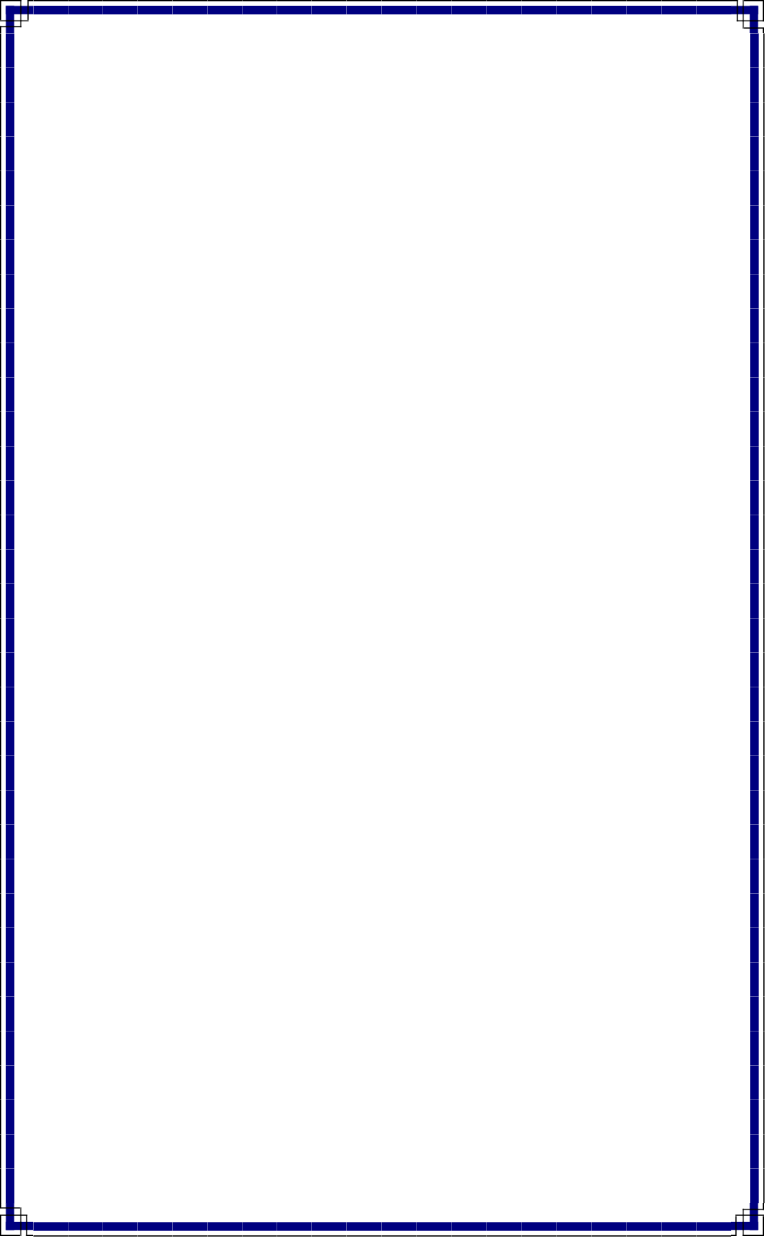
\includegraphics[width=\paperwidth,height=\paperheight]{images/vien.png}};
        \end{tikzpicture}
    }
    \begin{center}
        \vspace*{0.5cm}
        
        {\Large % Tăng từ \large lên \Large (khoảng 17pt)
        BỘ GIÁO DỤC VÀ ĐÀO TẠO\\
        TRƯỜNG ĐẠI HỌC ĐỒNG THÁP\\
        KHOA CÔNG NGHỆ VÀ KỸ THUẬT\\[0.2cm]
        \rule{5.5cm}{0.5pt}
        }
        
        \vspace{1.5cm}
        
        
\includegraphics[width=0.35\textwidth]{images/logo.png} % Phóng to logo một chút
        
        \vspace{1.5cm}
        
        {\LARGE \textbf{ % Tăng từ \Large lên \LARGE (khoảng 20pt) và thêm in đậm
        XÂY DỰNG WEBSITE BÁN DỊCH VỤ CLOUD\\
        VỚI ASP.NET CORE VÀ NEXT.JS\\
        }}
        
        \vspace{1.5cm}
        
        {\large % Tăng từ \normalsize lên \large (khoảng 14.4pt)
        Ngành: Khoa học máy tính\\[0.2cm]
        Tên học phần: Phát triển phần mềm hướng đối tượng\\[0.2cm]
        Mã học phần: IN421101\\
        }
        
        \vspace{2cm}
        
        {\large % Tăng từ \normalsize lên \large
        \begin{tabular}{ll}
            Nhóm thực hiện: & Nhóm 7 \\[0.2cm]
            Lớp: & 002341480101A \\[0.2cm]
            Giảng viên hướng dẫn: & Lê Minh Hiếu \\
        \end{tabular}
        }
        
        \vfill
        
        {\large % Tăng từ \normalsize lên \large
        Đồng Tháp, tháng 8 năm 2026
        }
        
    \end{center}
\end{titlepage}



% Lời cảm ơn
\chapter*{Lời Cảm Ơn}
\addcontentsline{toc}{chapter}{LỜI CẢM ƠN}

Lời đầu tiên, nhóm chúng em xin gửi lời cảm ơn chân thành và sâu sắc nhất đến \textbf{thầy Lê Minh Hiếu} đã tận tình giảng dạy, truyền đạt những kiến thức quý báu về Phát triển phần mềm hướng đối tượng trong suốt học kỳ vừa qua. Những bài giảng về Clean Architecture, Design Patterns, Unit Testing và quy trình CI/CD đã trở thành nền tảng vững chắc để nhóm có thể hoàn thành đồ án này.Hiếu

Chúng em cũng xin cảm ơn \textbf{Khoa Công nghệ và Kỹ thuật -- Trường Đại học Đồng Tháp} đã tạo điều kiện thuận lợi về cơ sở vật chất và môi trường học tập, giúp chúng em có không gian phát triển kỹ năng lập trình thực tế.

Cuối cùng, chúng em xin gửi lời cảm ơn đến tất cả các thành viên trong nhóm đã cùng nhau nỗ lực, phối hợp chặt chẽ và không ngừng học hỏi để hoàn thành dự án đúng tiến độ.

Mặc dù đã cố gắng hết sức, báo cáo chắc chắn không tránh khỏi những thiếu sót. Nhóm chúng em rất mong nhận được sự góp ý từ quý thầy cô để hoàn thiện hơn trong tương lai.

\begin{flushright}
\textit{Đồng Tháp, tháng 8 năm 2026}\\
\textbf{Nhóm 7}
\end{flushright}


% Danh sách thành viên
\chapter*{Danh Sách Thành Viên Nhóm}
\addcontentsline{toc}{chapter}{DANH SÁCH THÀNH VIÊN NHÓM}

\vspace{1cm}

\begin{center}
    \renewcommand{\arraystretch}{2} % Tăng khoảng cách dòng để dễ viết tay hoặc nhập chữ
    \begin{tabular}{|c|p{6cm}|p{4cm}|p{4cm}|}
        \hline
        \textbf{STT} & \textbf{Họ và tên} & \textbf{Mã sinh viên} & \textbf{Ghi chú} \\
        \hline
        1 & Nguyễn Trung Hậu & 0023411914 & Nhóm trưởng\\
        \hline
        2 & Lương Quang Khải  & 0022412375 & \\
        \hline
        3 & Võ Phụng Tiên & 0022410955 & \\
        \hline
        4 & Phan Thành Vinh & 0023412001 & \\
        \hline
    \end{tabular}
\end{center}


% Mục lục
\tableofcontents
\cleardoublepage

% Mục lục hình ảnh
\listoffigures
\cleardoublepage

% Mục lục từ viết tắt
\chapter*{Mục Lục Từ Viết Tắt}
\addcontentsline{toc}{chapter}{MỤC LỤC TỪ VIẾT TẮT}

\begin{itemize}
    \item \textbf{API} (Application Programming Interface): Giao diện lập trình ứng dụng.
    \item \textbf{CI/CD} (Continuous Integration/Continuous Deployment): Tích hợp liên tục và Triển khai liên tục.
    \item \textbf{ERD} (Entity-Relationship Diagram): Sơ đồ thực thể liên kết.
    \item \textbf{JWT} (JSON Web Token): Tiêu chuẩn mở an toàn cho việc truyền thông tin.
    \item \textbf{ORM} (Object-Relational Mapping): Kỹ thuật ánh xạ đối tượng với dữ liệu quan hệ.
    \item \textbf{SOLID}: Tập hợp 5 nguyên lý thiết kế hướng đối tượng.
    \item \textbf{VPS} (Virtual Private Server): Máy chủ riêng ảo.
    \item \textbf{SLA} (Service Level Agreement): Cam kết mức độ dịch vụ.
\end{itemize}


% ------------------- PHẦN NỘI DUNG -------------------
% Thiết lập Header, Footer cho toàn bộ văn bản có đánh số trang
\pagestyle{fancy}
\fancyhf{}
\fancyheadoffset{0pt}
\fancyfootoffset{0pt}
\setlength{\headwidth}{\textwidth}
\fancyhead[L]{BÁO CÁO BÀI TẬP LỚN: WEBSITE BÁN DỊCH VỤ CLOUD} % Header trái
\fancyfoot[L]{Người thực hiện: Nhóm 7} % Footer trái
\fancyfoot[R]{\thepage} % Số trang
\renewcommand{\headrulewidth}{0.4pt}
\renewcommand{\footrulewidth}{0.4pt}

\fancypagestyle{plain}{ % Áp dụng Header/Footer cho cả trang bắt đầu chương
  \fancyhf{}
  \fancyheadoffset{0pt}
  \fancyfootoffset{0pt}
  \fancyhead[L]{BÁO CÁO BÀI TẬP LỚN: WEBSITE BÁN DỊCH VỤ CLOUD}
  \fancyfoot[L]{Người thực hiện: Nhóm 7}
  \fancyfoot[R]{\thepage}
  \renewcommand{\headrulewidth}{0.4pt}
  \renewcommand{\footrulewidth}{0.4pt}
}

% Mở đầu (Bắt đầu đánh số trang, dùng số La Mã cho phần trước chương 1)
\pagenumbering{roman}
\chapter*{Mở Đầu}
\addcontentsline{toc}{chapter}{MỞ ĐẦU}

\section*{1. Bối cảnh đề tài}
Sự phát triển mạnh mẽ của công nghệ điện toán đám mây (Cloud Computing) đã thúc đẩy quá trình chuyển đổi số của các doanh nghiệp. Các dịch vụ như VPS (Máy chủ ảo), Hosting, Domain, Email doanh nghiệp hay bảo mật Firewall không còn xa lạ mà trở thành nền tảng thiết yếu cho bất kỳ doanh nghiệp nào muốn hiện diện và vận hành trên không gian mạng. Để đáp ứng nhu cầu đó, các nhà cung cấp dịch vụ Cloud cần có một hệ thống website chuyên nghiệp, ổn định để quảng bá dịch vụ, hỗ trợ khách hàng đăng ký và quản trị hệ thống một cách hiệu quả.

Nhận thấy tầm quan trọng của hệ thống website này, nhóm chúng em đã quyết định chọn đề tài: \textbf{"Xây dựng Website bán dịch vụ Cloud"}. Đồ án tập trung vào việc áp dụng các kiến thức cốt lõi của học phần Phát triển phần mềm hướng đối tượng để thiết kế và xây dựng một hệ thống hoàn chỉnh từ Backend đến Frontend, đáp ứng các tiêu chuẩn công nghiệp hiện đại.

\section*{2. Mục tiêu nghiên cứu}
Đồ án đặt ra các mục tiêu chính sau đây:
\begin{itemize}
    \item Ứng dụng mô hình \textbf{Clean Architecture} cùng các nguyên lý \textbf{SOLID} và \textbf{Design Patterns} (như Repository, Unit of Work) vào xây dựng Backend Web API bằng nền tảng ASP.NET Core 9.
    \item Phát triển giao diện người dùng hiện đại, tốc độ cao (Frontend) bằng công nghệ \textbf{Next.js} có khả năng hiển thị tương thích trên nhiều thiết bị (responsive).
    \item Triển khai các tính năng cốt lõi cho một website bán dịch vụ: Hiển thị bảng giá dịch vụ (VPS, Hosting, v.v.), tiếp nhận đơn đặt hàng, quản trị người dùng, hệ thống bảo mật bằng JWT và quản lý mã khuyến mãi.
    \item Vận dụng các quy trình làm việc nhóm hiệu quả thông qua Git/GitHub, thực hành viết \textbf{Unit Test}, xây dựng pipeline \textbf{CI/CD} và đóng gói ứng dụng bằng \textbf{Docker}.
\end{itemize}

\section*{3. Đối tượng và phạm vi nghiên cứu}
\textbf{Đối tượng nghiên cứu:}
\begin{itemize}
    \item Kiến trúc phần mềm và các mẫu thiết kế hướng đối tượng.
    \item Nền tảng .NET Core và công nghệ Next.js (React).
    \item Các quy trình phát triển và kiểm thử phần mềm tự động.
\end{itemize}
\textbf{Phạm vi nghiên cứu:} Đồ án tập trung xây dựng trang giới thiệu công khai (Landing Page) cho khách hàng và khu vực quản trị (Admin Dashboard) dành riêng cho quản trị viên với các nghiệp vụ quản lý gói dịch vụ, đơn hàng và tin tức nội bộ.

\section*{4. Cấu trúc của báo cáo}
Báo cáo được chia thành 5 chương chính:
\begin{itemize}
    \item \textbf{Chương I: Cơ sở lý thuyết và công nghệ áp dụng} -- Trình bày tổng quan về điện toán đám mây, các công nghệ Backend (ASP.NET Core, EF Core), Frontend (Next.js, Tailwind CSS) và cơ chế xác thực JWT.
    \item \textbf{Chương II: Phân tích yêu cầu hệ thống} -- Xác định tác nhân, yêu cầu chức năng (Landing Page và Admin Dashboard), yêu cầu phi chức năng, sơ đồ Use Case và Activity Diagram.
    \item \textbf{Chương III: Thiết kế hệ thống} -- Mô tả kiến trúc Clean Architecture 4 tầng, thiết kế cơ sở dữ liệu (ERD), các Design Patterns (Repository, Unit of Work) và Sequence Diagram.
    \item \textbf{Chương IV: Xây dựng và kiểm thử hệ thống} -- Trình bày giao diện người dùng thực tế, kết quả Unit Test (16 test cases) và hệ thống CI/CD, Docker.
    \item \textbf{Chương V: Kết luận và hướng phát triển} -- Đánh giá kết quả đạt được, phân công công việc của từng thành viên và định hướng phát triển tương lai.
\end{itemize}


% Các chương chính
\cleardoublepage
\pagenumbering{arabic} % Đánh số trang bắt đầu từ 1 cho Chương 1
\chapter{CƠ SỞ LÝ THUYẾT VÀ CÔNG NGHỆ ÁP DỤNG}

\section{Tổng quan về Điện toán đám mây (Cloud Computing)}
Điện toán đám mây là mô hình cung cấp các tài nguyên máy tính (máy chủ, mạng, lưu trữ, cơ sở dữ liệu, phần mềm) qua Internet (``đám mây'') nhằm cung cấp sự đổi mới nhanh hơn, tài nguyên linh hoạt và lợi thế kinh tế theo quy mô. 

Trong khuôn khổ của hệ thống bán dịch vụ Cloud, các khái niệm dịch vụ chính được hệ thống cung cấp bao gồm:
\begin{itemize}
    \item \textbf{VPS (Virtual Private Server):} Máy chủ riêng ảo được phân chia từ một máy chủ vật lý, cung cấp tài nguyên độc lập, có hệ điều hành riêng và cho phép toàn quyền quản trị (Root/Administrator).
    \item \textbf{Web Hosting:} Dịch vụ lưu trữ dữ liệu website trên máy chủ đã được cấu hình sẵn môi trường (web server, database server), giúp khách hàng dễ dàng đưa website lên Internet mà không cần kiến thức quản trị máy chủ sâu sắc.
    \item \textbf{Tên miền (Domain Name):} Địa chỉ định danh của một website trên mạng Internet, đóng vai trò như ``địa chỉ nhà'' thay thế cho dãy địa chỉ IP phức tạp.
\end{itemize}

\section{Nền tảng và Công nghệ phía Backend}

\subsection{ASP.NET Core và C\#}
ASP.NET Core \cite{microsoft_docs} là một framework mã nguồn mở, đa nền tảng do Microsoft phát triển dùng để xây dựng các ứng dụng web hiện đại, các dịch vụ IoT và các backend dùng cho ứng dụng di động. ASP.NET Core có hiệu năng rất cao, thiết kế theo mô hình mô-đun (modular) và hỗ trợ tích hợp sẵn Dependency Injection. 

Trong dự án này, ASP.NET Core 9 Web API được sử dụng để phát triển RESTful API phục vụ cho quá trình trao đổi dữ liệu với Frontend. API được chia thành hai nhóm chính: \texttt{Public API} (không yêu cầu đăng nhập) và \texttt{Admin API} (yêu cầu xác thực JWT và phân quyền Role).

\subsection{Entity Framework Core (EF Core)}
EF Core là một Object-Relational Mapper (ORM) nhẹ, mã nguồn mở, giúp lập trình viên C\# làm việc với cơ sở dữ liệu quan hệ bằng cách sử dụng các đối tượng .NET mạnh mẽ mà không cần phải viết phần lớn các câu truy vấn cơ sở dữ liệu thông thường. Hệ thống sử dụng EF Core kết hợp với SQL Server 2022 để lưu trữ và truy xuất dữ liệu. Quá trình quản lý sự thay đổi cấu trúc bảng được thực hiện thông qua cơ chế \textbf{Migrations} tự động.

\subsection{SQL Server 2022}
Microsoft SQL Server là hệ quản trị cơ sở dữ liệu quan hệ (RDBMS) được sử dụng rộng rãi trong môi trường doanh nghiệp. Trong dự án, SQL Server 2022 phiên bản Express được triển khai thông qua Docker container, giúp nhất quán môi trường phát triển giữa các thành viên trong nhóm.

\section{Nền tảng và Công nghệ phía Frontend}

\subsection{Next.js và React}
Next.js \cite{nextjs_docs} là một framework của React giúp xây dựng các ứng dụng web tối ưu hóa SEO thông qua khả năng Server-Side Rendering (SSR) và Static Site Generation (SSG). Next.js sử dụng kiến trúc App Router mới (từ phiên bản 13 trở lên), giúp cấu trúc thư mục logic hơn và hỗ trợ các tính năng React Server Components.

Trong dự án, Next.js được sử dụng để xây dựng toàn bộ giao diện người dùng bao gồm: Landing Page công khai (10 trang), Admin Dashboard (8 trang quản trị), và Customer Dashboard.

\subsection{Tailwind CSS}
Tailwind CSS là một utility-first CSS framework giúp xây dựng các giao diện người dùng nhanh chóng mà không cần phải thoát ra khỏi tệp HTML/JSX. Nó cung cấp các class mức độ thấp để kết hợp lại tạo thành bất kỳ thiết kế tùy chỉnh nào. Giao diện trang chủ và trang quản trị của dự án được thiết kế hoàn toàn bằng Tailwind CSS, mang lại vẻ ngoài hiện đại và thân thiện với thiết bị di động (Responsive Design).

\subsection{Axios và Quản lý Token}
Thư viện Axios được sử dụng để thực hiện các HTTP Request từ Frontend đến Backend API. Hệ thống cấu hình một \texttt{apiClient} tập trung với:
\begin{itemize}
    \item \texttt{baseURL}: trỏ đến địa chỉ Backend API (\texttt{http://localhost:5023/api}).
    \item \texttt{Interceptor Request}: tự động gắn JWT Token vào tiêu đề \texttt{Authorization} của mọi request.
    \item \texttt{Interceptor Response}: xử lý lỗi 401 (Unauthorized) bằng cách xóa token cũ và chuyển hướng về trang đăng nhập.
\end{itemize}

\section{Xác thực và Bảo mật với JWT (JSON Web Token)}
JSON Web Token (JWT) là một tiêu chuẩn mở (RFC 7519) định nghĩa một cách nhỏ gọn và tự chứa để truyền tải thông tin an toàn giữa các bên dưới dạng một đối tượng JSON. Thông tin này có thể được xác minh và tin cậy vì nó được ký điện tử.

Trong hệ thống, JWT được ứng dụng làm cơ chế xác thực chính (Stateless Authentication):
\begin{enumerate}
    \item Quản trị viên gửi yêu cầu đăng nhập (email và mật khẩu) lên Backend qua endpoint \texttt{POST /api/auth/login}.
    \item Backend kiểm tra mật khẩu đã mã hóa bằng thuật toán \textbf{BCrypt}, nếu đúng sẽ sinh ra một chuỗi JWT (\texttt{AccessToken}) có chứa thông tin cơ bản (ID người dùng, Role) cùng với chữ ký bí mật, và một \texttt{RefreshToken} để gia hạn phiên làm việc.
    \item Frontend lưu token vào Cookie và gửi kèm trong tiêu đề \texttt{Authorization: Bearer <token>} của các yêu cầu tiếp theo.
    \item Backend xác minh chữ ký của JWT thông qua Middleware; nếu hợp lệ, yêu cầu được cấp phép thực hiện theo phân quyền tương ứng (\texttt{Admin} hoặc \texttt{Editor}).
\end{enumerate}

\section{Các nguyên lý thiết kế SOLID}
SOLID là tập hợp 5 nguyên lý thiết kế hướng đối tượng giúp tạo ra phần mềm linh hoạt, dễ bảo trì và mở rộng:

\begin{itemize}
    \item \textbf{S -- Single Responsibility Principle:} Mỗi lớp chỉ chịu trách nhiệm cho một chức năng duy nhất. Ví dụ: \texttt{OrderService} chỉ xử lý logic đơn hàng, \texttt{JwtService} chỉ xử lý việc tạo/xác thực token.
    \item \textbf{O -- Open/Closed Principle:} Hệ thống mở cho việc mở rộng nhưng đóng cho việc sửa đổi. Ví dụ: thêm một dịch vụ mới (SSL, Firewall) chỉ cần tạo thêm bản ghi trong bảng \texttt{ServiceCategory} mà không cần sửa code.
    \item \textbf{L -- Liskov Substitution Principle:} Các lớp triển khai (Implementation) có thể thay thế cho lớp cha (Interface) mà không ảnh hưởng logic. Ví dụ: \texttt{OrderService} triển khai giao diện \texttt{IOrderService}, có thể thay bằng \texttt{MockOrderService} khi test.
    \item \textbf{I -- Interface Segregation Principle:} Hệ thống sử dụng 9 giao diện chuyên biệt (\texttt{IOrderService}, \texttt{ICategoryService}, \texttt{INewsArticleService}...) thay vì một giao diện lớn chứa tất cả.
    \item \textbf{D -- Dependency Inversion Principle:} Các lớp cấp cao (Controller, Service) phụ thuộc vào giao diện trừu tượng (Interface) thay vì lớp cụ thể. Việc ``nối dây'' (wiring) được thực hiện tại \texttt{Program.cs} thông qua Dependency Injection container có sẵn của ASP.NET Core.
\end{itemize}

\section{Các công cụ hỗ trợ phát triển}
\begin{itemize}
    \item \textbf{Git \& GitHub:} Quản lý phiên bản mã nguồn, làm việc nhóm qua Pull Request.
    \item \textbf{Docker \& Docker Compose:} Đóng gói ứng dụng và cơ sở dữ liệu vào container.
    \item \textbf{GitHub Actions:} Pipeline CI tự động build và chạy unit test khi push/PR.
    \item \textbf{xUnit \& Moq:} Framework kiểm thử đơn vị và thư viện mock cho .NET.
    \item \textbf{Swagger (OpenAPI):} Tự động tạo tài liệu API tương tác cho Backend.
    \item \textbf{QRCoder:} Thư viện .NET sinh mã QR Code cho từng gói dịch vụ.
    \item \textbf{ClosedXML:} Thư viện .NET xuất dữ liệu ra file Excel (.xlsx).
\end{itemize}

\chapter{PHÂN TÍCH YÊU CẦU HỆ THỐNG}

\section{Xác định tác nhân (Actors)}
Trong hệ thống website cung cấp dịch vụ Cloud, có hai tác nhân chính tham gia tương tác với hệ thống:
\begin{itemize}
    \item \textbf{Khách hàng (Customer):} Là người dùng truy cập vào website để xem thông tin dịch vụ, so sánh bảng giá, đặt mua dịch vụ (VPS, Hosting, Domain, v.v.) và đăng ký trở thành đối tác liên kết (Affiliate).
    \item \textbf{Quản trị viên (Admin/Editor):} Là nhân viên của công ty cung cấp dịch vụ, có nhiệm vụ cấu hình bảng giá, quản lý các danh mục dịch vụ, xử lý/duyệt đơn đặt hàng từ khách hàng, quản lý chương trình khuyến mãi, xuất báo cáo doanh thu và đăng tải bài viết/tin tức. Hệ thống phân quyền thành 2 role: \texttt{Admin} (toàn quyền) và \texttt{Editor} (quyền hạn chế, chỉ quản lý nội dung).
\end{itemize}

\section{Yêu cầu chức năng}

\subsection{Chức năng trang công khai (Landing Page)}
Bảng~\ref{tab:func_public} liệt kê đầy đủ các chức năng của trang công khai mà khách hàng có thể truy cập mà không cần đăng nhập.

\begin{table}[htbp]
    \centering
    \caption{Bảng chức năng trang công khai (Landing Page)}
    \label{tab:func_public}
    \begin{tabular}{|c|p{3cm}|p{9cm}|}
        \hline
        \textbf{STT} & \textbf{Chức năng} & \textbf{Mô tả chi tiết} \\
        \hline
        1 & Trang chủ & Hero banner giới thiệu, hiển thị danh mục dịch vụ nổi bật (lấy từ API), cam kết Uptime 99.99\%, tin tức mới nhất, testimonials khách hàng. \\
        \hline
        2 & Giới thiệu & Lịch sử công ty, hạ tầng datacenter, các chứng chỉ (ISO), cam kết SLA/Uptime 99.99\%, đội ngũ kỹ thuật. \\
        \hline
        3 & Dịch vụ & Danh mục: VPS, Hosting, Domain, Email doanh nghiệp, SSL, Firewall chống DDoS. Mỗi dịch vụ kèm mô tả và thông số kỹ thuật chi tiết. \\
        \hline
        4 & Bảng giá & So sánh các gói theo cấu hình (CPU/RAM/SSD/Băng thông). Chuyển đổi giá theo chu kỳ Tháng/Năm (toggle). Hiển thị mã QR cho từng gói dịch vụ. \\
        \hline
        5 & Khách hàng & Đánh giá/testimonial từ khách hàng, logo đối tác tiêu biểu. \\
        \hline
        6 & Tin tức / Blog & Danh sách bài viết với phân trang, tìm kiếm theo từ khóa, phân loại (hướng dẫn, khuyến mãi). Trang chi tiết bài viết theo slug. \\
        \hline
        7 & Liên hệ / Đặt DV & Form đăng ký: chọn chủ đề dịch vụ, nhập thông tin khách hàng. Dữ liệu được lưu vào Database qua API. \\
        \hline
        8 & Đối tác / Affiliate & Trang thông tin chính sách hoa hồng, danh sách đối tác chiến lược. Form đăng ký làm đối tác/affiliate gửi qua API. \\
        \hline
    \end{tabular}
\end{table}

\subsection{Chức năng trang quản trị (Admin Dashboard)}
Bảng~\ref{tab:func_admin} liệt kê các chức năng quản trị, yêu cầu đăng nhập JWT và phân quyền Role.

\begin{table}[htbp]
    \centering
    \caption{Bảng chức năng trang quản trị (Admin Dashboard)}
    \label{tab:func_admin}
    \begin{tabular}{|c|p{3.5cm}|p{6cm}|p{2.5cm}|}
        \hline
        \textbf{STT} & \textbf{Chức năng} & \textbf{Mô tả chi tiết} & \textbf{Role} \\
        \hline
        1 & Đăng nhập, Refresh Token, Đổi mật khẩu & Xác thực bằng JWT. Hỗ trợ Refresh Token gia hạn phiên và đổi mật khẩu cho tài khoản đang đăng nhập. & Tất cả \\
        \hline
        2 & CRUD Gói dịch vụ & Thêm, sửa, xóa các gói dịch vụ (CPU, RAM, Disk, giá). Tự động cập nhật giá trên trang công khai. & Admin \\
        \hline
        3 & CRUD Danh mục DV + Sinh QR & Quản lý danh mục (VPS, Hosting, Domain). Sinh mã QR cho từng gói, quét ra trang chi tiết. & Admin \\
        \hline
        4 & CRUD Tin tức/Blog & Soạn thảo, chỉnh sửa, xóa tin tức. Hỗ trợ gắn slug URL. & Admin, Editor \\
        \hline
        5 & Quản lý Đơn hàng + Affiliate & Xem danh sách, đổi trạng thái (Mới $\rightarrow$ Đang xử lý $\rightarrow$ Hoàn tất/Từ chối). & Admin, Editor \\
        \hline
        6 & CRUD Khuyến mãi & Thêm, sửa, xóa chương trình khuyến mãi với mã code, phần trăm giảm giá, thời hạn. & Admin \\
        \hline
        7 & Thống kê biểu đồ & Tổng quan: số đơn hàng, doanh thu theo tháng, gói dịch vụ được quan tâm. Biểu đồ trực quan. & Admin \\
        \hline
        8 & Xuất Excel & Xuất danh sách yêu cầu đặt dịch vụ ra file Excel (.xlsx) qua thư viện ClosedXML. & Admin \\
        \hline
        9 & Audit Log & Ghi lại lịch sử: ai đăng nhập, ai sửa giá, khi nào. Hiển thị dạng bảng có phân trang. & Admin \\
        \hline
    \end{tabular}
\end{table}

\section{Yêu cầu phi chức năng}
\begin{itemize}
    \item \textbf{Giao diện (UI/UX):} Website phải có thiết kế hiện đại, tốc độ phản hồi nhanh (dưới 3 giây) và hiển thị tốt trên cả nền tảng Desktop và Mobile (Responsive). Menu điều hướng hỗ trợ Hamburger menu trên thiết bị di động.
    \item \textbf{Bảo mật:} Mật khẩu phải được mã hóa bằng thuật toán BCrypt trước khi lưu trữ. Các API quản trị yêu cầu xác thực JWT nghiêm ngặt với phân quyền theo Role (\texttt{[Authorize(Roles = "Admin")]}).
    \item \textbf{Kiến trúc:} Hệ thống được xây dựng theo mô hình Clean Architecture 4 tầng, đảm bảo tính tách biệt (Separation of Concerns) giữa các module.
    \item \textbf{Tính sẵn sàng và mở rộng:} Hệ thống được đóng gói bằng Docker, chỉ cần một lệnh \texttt{docker compose up} là có thể triển khai trên mọi hệ điều hành.
    \item \textbf{Kiểm thử:} Tối thiểu 15 unit test cases sử dụng xUnit và Moq, đảm bảo tính đúng đắn của logic nghiệp vụ tại tầng Application.
\end{itemize}

\section{Sơ đồ Use Case (Ca sử dụng)}
Sơ đồ Use Case tổng quát giúp hình dung rõ bức tranh toàn cảnh về cách các tác nhân tương tác với hệ thống. Khách hàng (Customer) tương tác với các trang công khai, còn Quản trị viên (Admin/Editor) tương tác với hệ thống quản trị sau khi xác thực JWT.

% TODO: Chèn ảnh Sơ đồ Use Case tổng quát. Hãy lưu file ảnh tên là 'use_case_diagram.png' vào thư mục 'images'
\begin{figure}[htbp]
    \centering
    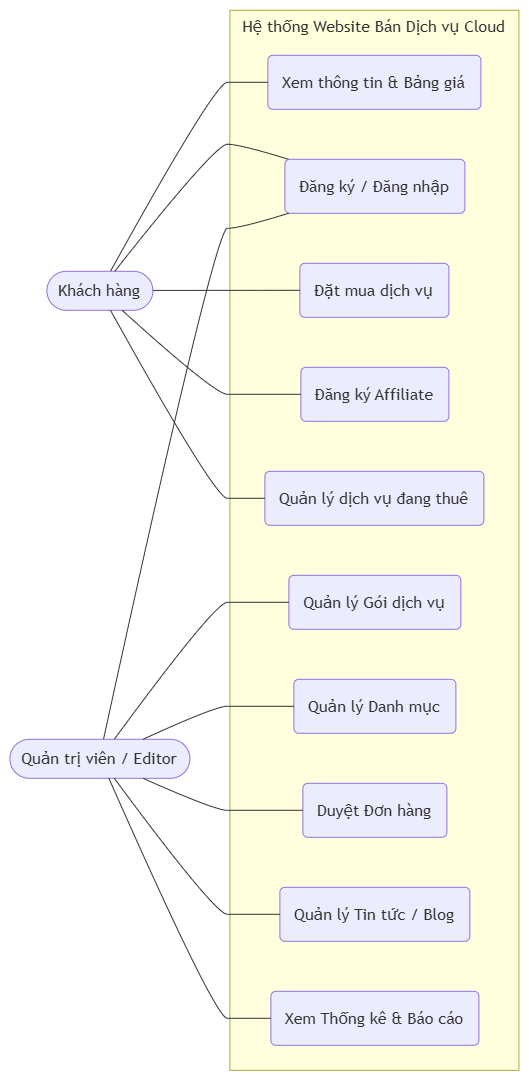
\includegraphics[width=0.7\textwidth]{images/use_case_diagram.png}
    \caption{Sơ đồ Use Case tổng quát của hệ thống Website bán dịch vụ Cloud}
    \label{fig:use_case}
\end{figure}

\section{Sơ đồ Hoạt động (Activity Diagram)}
Để làm rõ luồng nghiệp vụ cốt lõi, Sơ đồ hoạt động sau đây minh họa quy trình ``Đặt hàng dịch vụ'' của một khách hàng từ lúc bắt đầu cho đến khi quản trị viên phê duyệt đơn hàng.

% TODO: Chèn ảnh Sơ đồ Hoạt động Đặt hàng. Hãy lưu file ảnh tên là 'activity_order.png' vào thư mục 'images'
\begin{figure}[htbp]
    \centering
    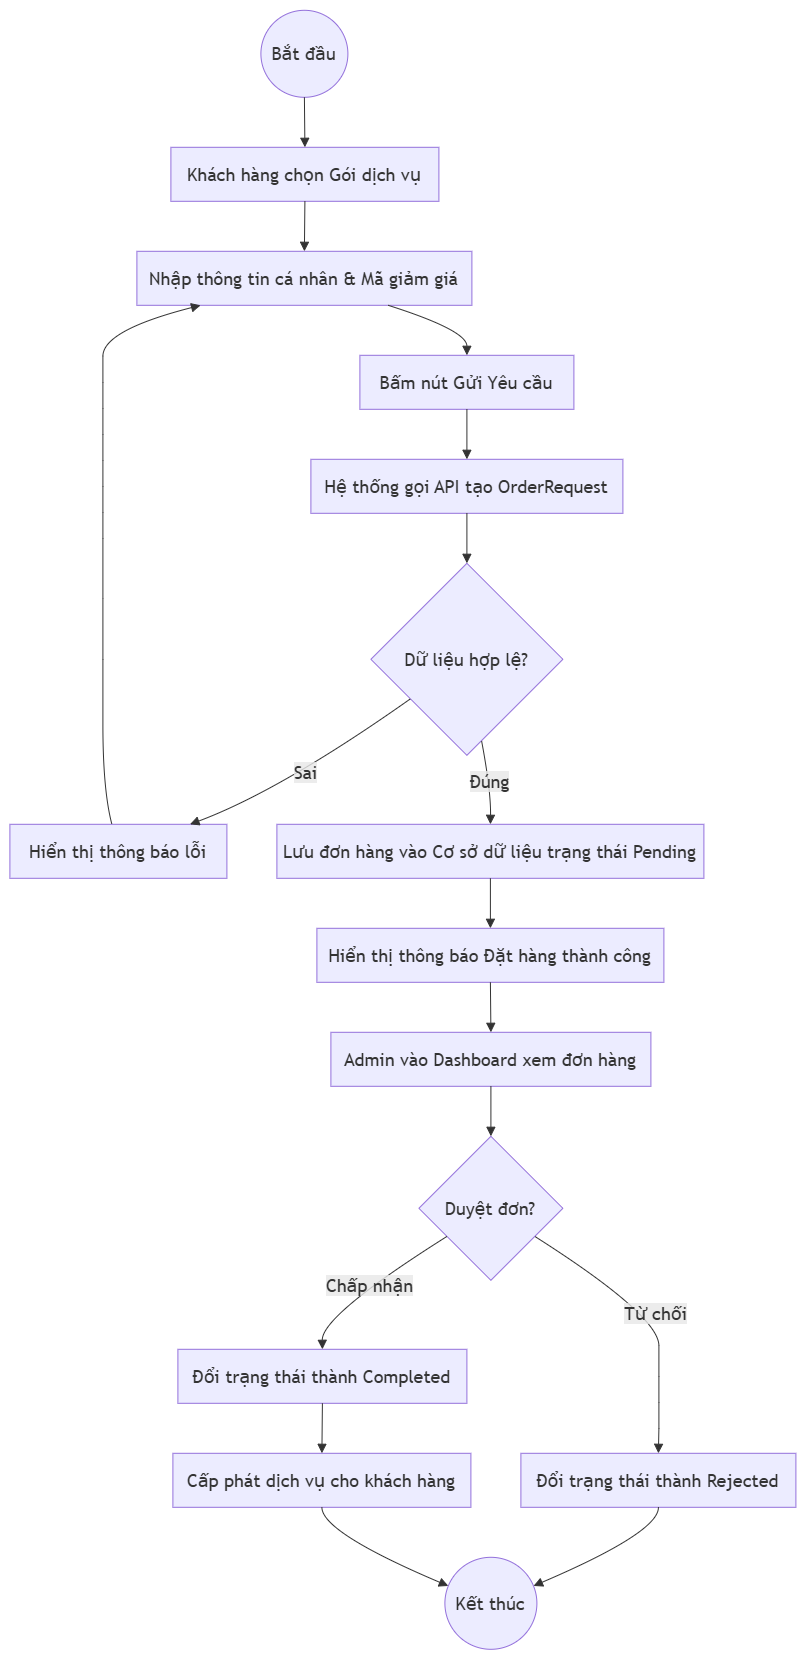
\includegraphics[width=0.7\textwidth]{images/activity_order.png}
    \caption{Sơ đồ Hoạt động nghiệp vụ Đặt hàng dịch vụ}
    \label{fig:activity_order}
\end{figure}

\chapter{THIẾT KẾ HỆ THỐNG}

\section{Thiết kế Kiến trúc (Architecture Design)}
Để đảm bảo hệ thống có khả năng bảo trì cao, dễ dàng mở rộng và độc lập với các thư viện hoặc cơ sở dữ liệu, dự án được xây dựng dựa trên nguyên lý của mô hình \textbf{Clean Architecture} \cite{cleanarchitecture}. Mã nguồn Backend chia thành 4 project (4 tầng đồng tâm):

\begin{enumerate}
    \item \textbf{CloudService.Domain (Core):} Chứa các logic nghiệp vụ cốt lõi, hoàn toàn thuần C\#. Gồm 9 thực thể (Entities), 3 Enums (\texttt{UserRole}, \texttt{OrderStatus}, \texttt{BillingCycle}), lớp cơ sở \texttt{BaseEntity} và các giao diện Repository. Lớp này \textbf{không tham chiếu} đến bất kỳ lớp nào khác.
    \item \textbf{CloudService.Application:} Đóng vai trò làm lớp trung gian (Use Cases), chứa 8 Services (\texttt{OrderService}, \texttt{CategoryService}, \texttt{NewsArticleService}, \texttt{ServicePlanService}, \texttt{AffiliateService}, \texttt{AuditLogService}, \texttt{AuthService}, \texttt{AdminStatsService}) cùng 9 giao diện (Interfaces) tương ứng và các DTOs (Data Transfer Objects).
    \item \textbf{CloudService.Infrastructure:} Thực thi (Implement) các giao diện được định nghĩa ở lớp Core. Chứa: \texttt{AppDbContext} (DbContext của EF Core), 7 Repository cụ thể, lớp \texttt{UnitOfWork}, và 5 Infrastructure Services (\texttt{JwtService}, \texttt{PasswordHashService}, \texttt{QrCodeService}, \texttt{ExcelExportService}, \texttt{AuthService}).
    \item \textbf{CloudService.WebApi (Presentation):} Là lớp giao tiếp với bên ngoài (Frontend). Chứa 14 Controllers (5 Public + 9 Admin), 2 Middleware (\texttt{ExceptionMiddleware}, \texttt{AuditMiddleware}) và cấu hình Dependency Injection tại \texttt{Program.cs}.
\end{enumerate}

% TODO: Chèn ảnh Sơ đồ kiến trúc hệ thống. Hãy lưu file ảnh tên là 'clean_architecture.png' vào thư mục 'images'
\begin{figure}[htbp]
    \centering
    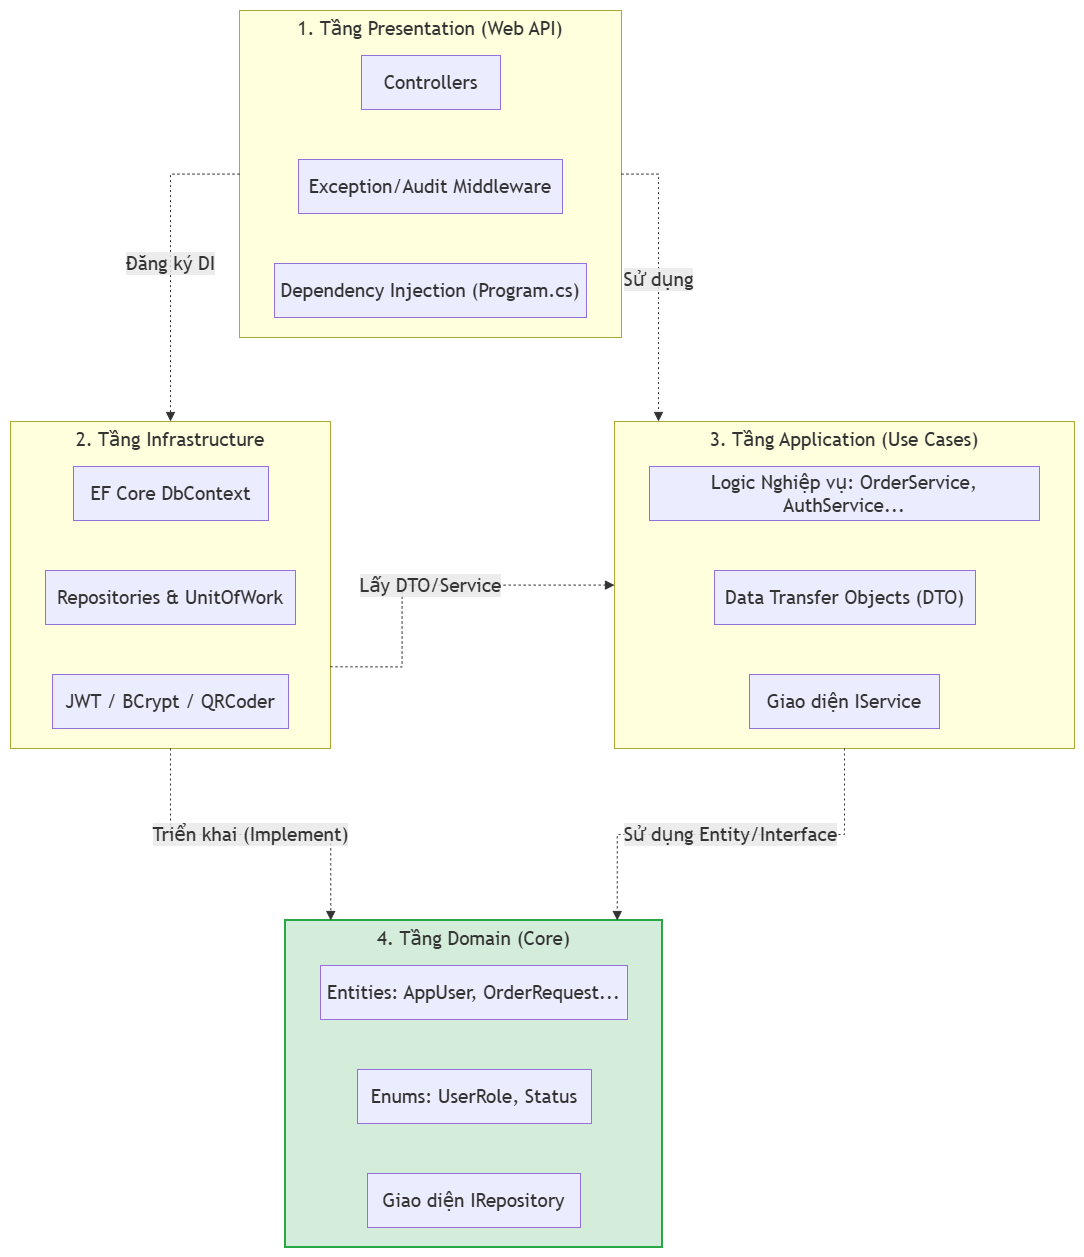
\includegraphics[width=0.9\textwidth]{images/clean_architecture.png}
    \caption{Sơ đồ khối Clean Architecture trong dự án}
    \label{fig:clean_arch}
\end{figure}

\section{Thiết kế Cơ sở dữ liệu (Database Design)}
Dữ liệu của hệ thống được thiết kế chặt chẽ và chuẩn hóa nhằm tránh dư thừa thông tin. Hệ thống sử dụng tổng cộng \textbf{10 bảng} (tương ứng 9 Entities + 1 bảng Role tích hợp Enum).

\subsection{Sơ đồ thực thể liên kết (ERD)}
% TODO: Chèn ảnh Sơ đồ ERD. Hãy lưu file ảnh tên là 'erd.png' vào thư mục 'images'
\begin{figure}[htbp]
    \centering
    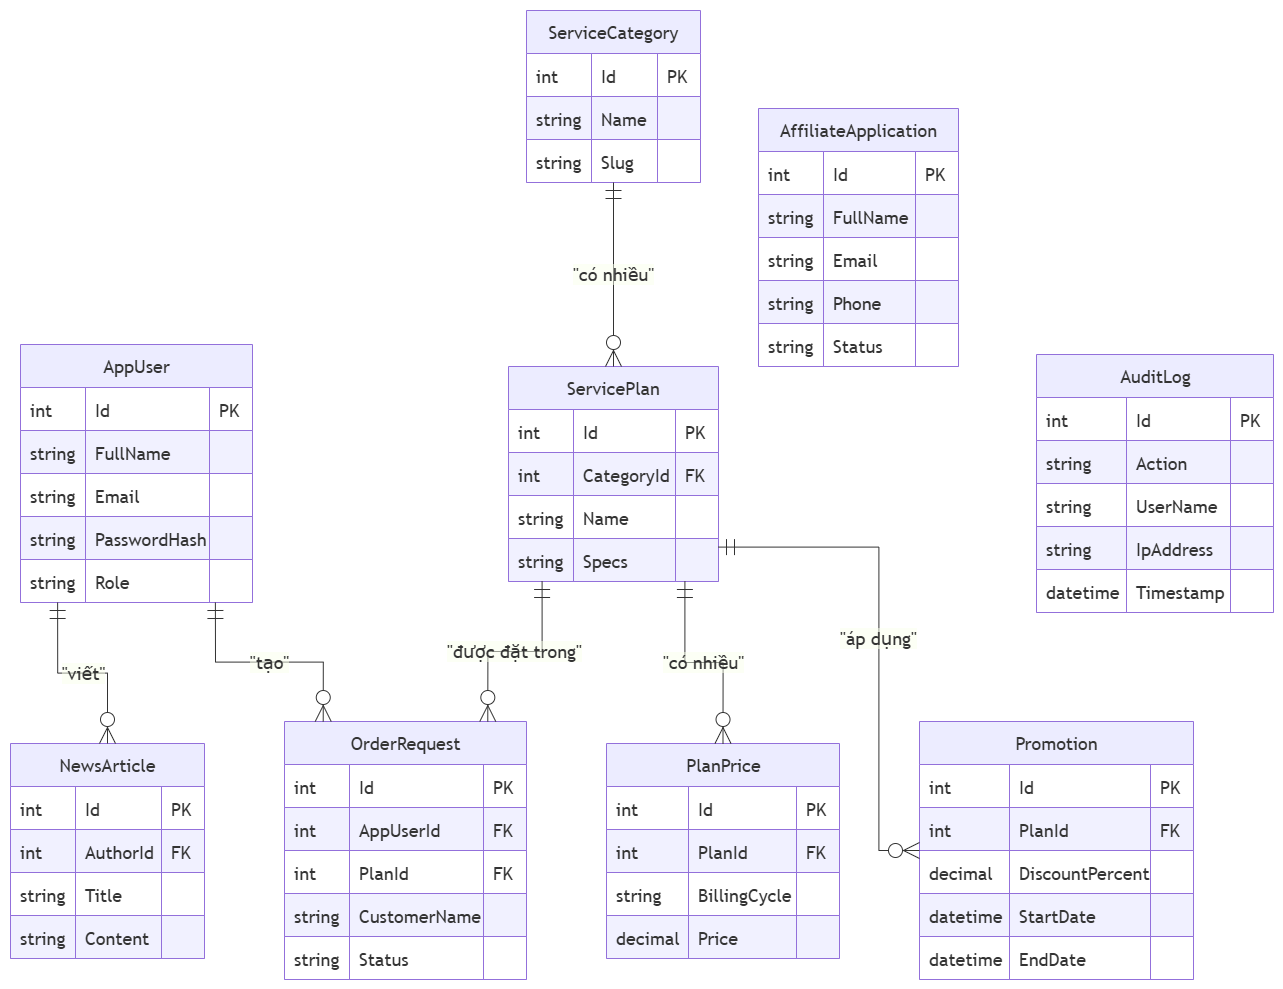
\includegraphics[width=1\textwidth]{images/erd.png}
    \caption{Sơ đồ thực thể liên kết (ERD)}
    \label{fig:erd}
\end{figure}

\subsection{Mô tả các thực thể (Entities) chính}
Bảng~\ref{tab:entities} mô tả chi tiết 9 thực thể chính được triển khai trong hệ thống, tất cả đều kế thừa từ \texttt{BaseEntity} (chứa \texttt{Id}, \texttt{CreatedAt}, \texttt{UpdatedAt}).

\begin{table}[htbp]
    \centering
    \caption{Danh sách các thực thể (Entities) trong hệ thống}
    \label{tab:entities}
    \begin{tabular}{|c|p{3.5cm}|p{8.5cm}|}
        \hline
        \textbf{STT} & \textbf{Entity} & \textbf{Mô tả và các thuộc tính chính} \\
        \hline
        1 & \texttt{ServiceCategory} & Danh mục dịch vụ gốc (VPS, Hosting, Domain). Thuộc tính: \texttt{Name}, \texttt{Slug}, \texttt{Description}. Quan hệ 1-N với \texttt{ServicePlan}. \\
        \hline
        2 & \texttt{ServicePlan} & Gói dịch vụ cụ thể. Thuộc tính: \texttt{Name}, \texttt{Slug}, \texttt{Specs} (CPU/RAM/SSD), \texttt{CategoryId}. Quan hệ N-1 với \texttt{ServiceCategory}, 1-N với \texttt{PlanPrice}. \\
        \hline
        3 & \texttt{PlanPrice} & Bảng giá theo chu kỳ. Thuộc tính: \texttt{BillingCycle} (Monthly/Yearly), \texttt{Price}, \texttt{PlanId}. Cho phép một gói có nhiều mức giá khác nhau. \\
        \hline
        4 & \texttt{Promotion} & Chương trình khuyến mãi. Thuộc tính: \texttt{PlanId}, \texttt{DiscountPercent}, \texttt{StartDate}, \texttt{EndDate}, \texttt{IsActive}. Quan hệ N-1 với \texttt{ServicePlan}. \\
        \hline
        5 & \texttt{NewsArticle} & Bài viết/Tin tức. Thuộc tính: \texttt{Title}, \texttt{Slug}, \texttt{Content} (HTML), \texttt{Summary}, \texttt{Category}, \texttt{AuthorId}. \\
        \hline
        6 & \texttt{OrderRequest} & Yêu cầu đặt dịch vụ. Thuộc tính: \texttt{CustomerName}, \texttt{Email}, \texttt{Phone}, \texttt{ServiceName}, \texttt{PlanId}, \texttt{BillingCycle}, \texttt{Status} (Enum: Pending/Processing/Completed/Rejected). \\
        \hline
        7 & \texttt{AffiliateApplication} & Đơn đăng ký đối tác. Thuộc tính: \texttt{FullName}, \texttt{Email}, \texttt{Phone}, \texttt{Website}, \texttt{Status}. \\
        \hline
        8 & \texttt{AppUser} & Tài khoản quản trị. Thuộc tính: \texttt{FullName}, \texttt{Email}, \texttt{PasswordHash}, \texttt{Role} (Enum: Admin/Editor), \texttt{RefreshToken}, \texttt{RefreshTokenExpiry}. \\
        \hline
        9 & \texttt{AuditLog} & Nhật ký hệ thống. Thuộc tính: \texttt{Action}, \texttt{UserName}, \texttt{IpAddress}, \texttt{Timestamp}, \texttt{Details}. \\
        \hline
    \end{tabular}
\end{table}

\section{Thiết kế RESTful API}
Backend cung cấp tổng cộng \textbf{37 endpoints} chia thành 3 nhóm chính. Bảng~\ref{tab:api_endpoints} liệt kê các endpoint tiêu biểu.

\begin{table}[htbp]
    \centering
    \caption{Danh sách các API Endpoint chính}
    \label{tab:api_endpoints}
    \begin{tabular}{|p{1.5cm}|p{5.5cm}|p{5cm}|}
        \hline
        \textbf{Method} & \textbf{Route} & \textbf{Mô tả} \\
        \hline
        \multicolumn{3}{|c|}{\textit{Public API (Không cần đăng nhập)}} \\
        \hline
        GET & \texttt{/api/public/service-categories} & Danh mục dịch vụ \\
        GET & \texttt{/api/public/service-plans} & Tất cả gói dịch vụ \\
        GET & \texttt{/api/public/service-plans/\{id\}/qr} & Mã QR cho gói DV \\
        GET & \texttt{/api/public/news} & Danh sách tin tức \\
        GET & \texttt{/api/public/news/\{slug\}} & Chi tiết bài viết \\
        POST & \texttt{/api/public/orders} & Gửi yêu cầu đặt DV \\
        POST & \texttt{/api/public/affiliates} & Đăng ký affiliate \\
        \hline
        \multicolumn{3}{|c|}{\textit{Auth API}} \\
        \hline
        POST & \texttt{/api/auth/login} & Đăng nhập $\rightarrow$ JWT \\
        POST & \texttt{/api/auth/refresh} & Gia hạn Access Token \\
        POST & \texttt{/api/auth/change-password} & Đổi mật khẩu \\
        \hline
        \multicolumn{3}{|c|}{\textit{Admin API (Yêu cầu JWT + Role)}} \\
        \hline
        CRUD & \texttt{/api/admin/service-plans} & Quản lý gói DV \\
        CRUD & \texttt{/api/admin/categories} & Quản lý danh mục \\
        CRUD & \texttt{/api/admin/news} & Quản lý tin tức \\
        CRUD & \texttt{/api/admin/promotions} & Quản lý khuyến mãi \\
        GET & \texttt{/api/admin/stats/summary} & Thống kê tổng quan \\
        GET & \texttt{/api/admin/export/orders} & Xuất Excel đơn hàng \\
        GET & \texttt{/api/admin/audit-logs} & Nhật ký hệ thống \\
        \hline
    \end{tabular}
\end{table}

\section{Thiết kế Mẫu thiết kế (Design Patterns)}
Các mẫu thiết kế (Design Patterns) \cite{gof} là những giải pháp tối ưu đã được kiểm chứng cho các vấn đề lặp lại trong thiết kế phần mềm. Dự án áp dụng các pattern sau:

\subsection{Repository Pattern}
Lớp \texttt{IGenericRepository<T>} cung cấp một tập hợp các hàm CRUD tiêu chuẩn chung cho mọi bảng. Các lớp nghiệp vụ chỉ cần gọi các phương thức như \texttt{GetAllAsync}, \texttt{GetByIdAsync} mà không cần biết chi tiết về câu lệnh SQL dưới tầng hạ tầng. Điều này giúp mã nguồn Application hoàn toàn không bị ``trói buộc'' với Entity Framework.

Trong dự án, 7 Repository cụ thể đã được triển khai: \texttt{ServiceCategoryRepository}, \texttt{ServicePlanRepository}, \texttt{NewsArticleRepository}, \texttt{OrderRequestRepository}, \texttt{AffiliateApplicationRepository}, \texttt{AppUserRepository}, \texttt{AuditLogRepository}.

\subsection{Unit of Work Pattern}
Khi có nhiều Repositories cần tương tác với Database cùng một lúc (ví dụ: tạo đơn hàng \texttt{OrderRequest} và cập nhật trạng thái affiliate), mô hình Unit of Work (giao diện \texttt{IUnitOfWork}) được sử dụng để gom các thao tác này vào chung một Giao dịch (Transaction). Lệnh \texttt{CompleteAsync()} đảm bảo dữ liệu chỉ được lưu nếu không xảy ra lỗi.

\subsection{Middleware Pattern}
Hệ thống sử dụng 2 Middleware tùy chỉnh theo dạng ``ống nước'' (Pipeline):
\begin{itemize}
    \item \texttt{ExceptionMiddleware}: Bắt toàn bộ exception chưa được xử lý và trả về response JSON chuẩn với mã lỗi HTTP phù hợp (400, 404, 500).
    \item \texttt{AuditMiddleware}: Tự động ghi lại mọi hành động quan trọng (đăng nhập, thay đổi dữ liệu) vào bảng \texttt{AuditLog} kèm thông tin IP, thời gian và người thực hiện.
\end{itemize}

\subsection{Dependency Injection (DI)}
Toàn bộ việc ``nối dây'' giữa các Interface và Implementation được cấu hình tập trung tại \texttt{Program.cs} thông qua DI container tích hợp sẵn của ASP.NET Core. Ví dụ:

\begin{verbatim}
builder.Services.AddScoped<IOrderService, OrderService>();
builder.Services.AddScoped<ICategoryService, CategoryService>();
builder.Services.AddScoped<IUnitOfWork, UnitOfWork>();
\end{verbatim}

\section{Sơ đồ Tuần tự (Sequence Diagram)}
Sơ đồ tuần tự thể hiện sự giao tiếp và thứ tự các thông điệp truyền đi giữa Client (Frontend) và Server (Backend) trong một chức năng. 

Dưới đây minh họa quy trình Đăng nhập và nhận JWT Token: Frontend gửi \texttt{POST /api/auth/login} $\rightarrow$ AuthController gọi AuthService $\rightarrow$ kiểm tra PasswordHash bằng BCrypt $\rightarrow$ JwtService sinh AccessToken + RefreshToken $\rightarrow$ trả về Frontend lưu Cookie.

% TODO: Chèn ảnh Sơ đồ Tuần tự quá trình Đăng nhập. Hãy lưu file ảnh tên là 'sequence_login.png' vào thư mục 'images'
\begin{figure}[htbp]
    \centering
    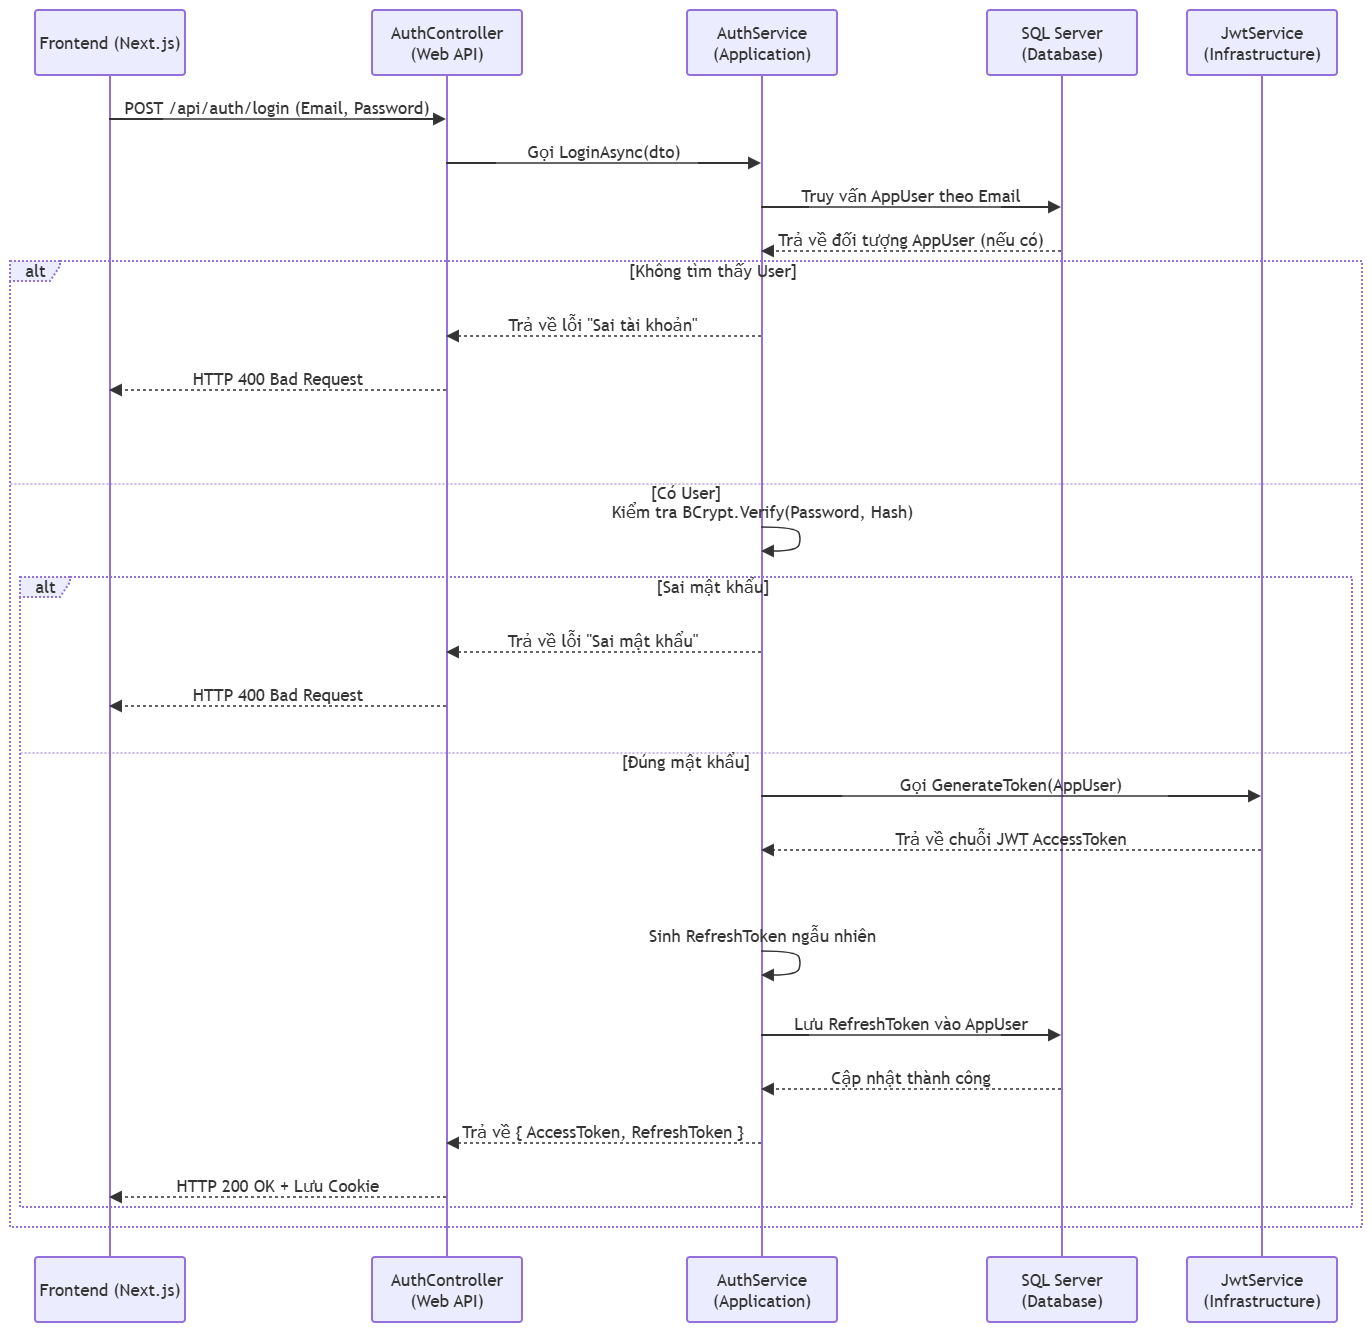
\includegraphics[width=0.9\textwidth]{images/sequence_login.png}
    \caption{Sơ đồ Tuần tự luồng xử lý xác thực đăng nhập cấp phát JWT}
    \label{fig:sequence_login}
\end{figure}

\chapter{XÂY DỰNG VÀ KIỂM THỬ HỆ THỐNG}

\section{Xây dựng Giao diện người dùng (UI)}
Giao diện của hệ thống được xây dựng hoàn toàn bằng Next.js (App Router) và Tailwind CSS, mang lại trải nghiệm mượt mà, phản hồi siêu tốc. Toàn bộ giao diện sử dụng thiết kế Responsive, tương thích trên cả Desktop và Mobile.

\subsection{Cấu trúc thư mục Frontend}
Mã nguồn Frontend được tổ chức theo kiến trúc App Router của Next.js:

\begin{verbatim}
frontend/src/
|-- app/
|   |-- (public)/          # 10 trang cong khai
|   |   |-- page.tsx       # Trang chu (SSR)
|   |   |-- bang-gia/      # Bang gia + QR
|   |   |-- tin-tuc/       # Tin tuc + [slug]
|   |   |-- dich-vu/       # Dich vu + [slug]
|   |   |-- lien-he/       # Form lien he -> API
|   |   |-- doi-tac/       # Form affiliate -> API
|   |   |-- Header.tsx     # Navbar + Hamburger
|   |   \-- Footer.tsx     # Footer
|   |-- admin/             # 8 trang quan tri
|   |   |-- dashboard/     # Thong ke tong quan
|   |   |-- services/      # CRUD goi dich vu
|   |   |-- news/          # CRUD tin tuc
|   |   |-- orders/        # Quan ly don hang
|   |   |-- promotions/    # CRUD khuyen mai
|   |   \-- audit-logs/    # Nhat ky he thong
|   \-- layout.tsx         # Root layout + SEO
|-- lib/axios.ts           # apiClient cau hinh
|-- middleware.ts          # Auth middleware
\-- types/index.ts         # TypeScript interfaces
\end{verbatim}

\subsection{Giao diện Landing Page công khai}
Trang Landing Page tập trung vào việc hiển thị các thông tin giới thiệu, các lợi thế cạnh tranh (như cam kết Uptime 99.99\%) và bảng giá dịch vụ để thu hút người mua.

Các trang công khai chính gồm: Trang chủ, Giới thiệu, Dịch vụ (danh sách + chi tiết theo slug), Bảng giá (toggle Tháng/Năm + mã QR), Khách hàng (testimonials), Tin tức (danh sách + chi tiết), Liên hệ (form gửi API) và Đối tác (form đăng ký affiliate).

% TODO: Chèn ảnh giao diện trang chủ. Hãy lưu file ảnh tên là 'landing_home.png' vào thư mục 'images'
\begin{figure}[htbp]
    \centering
    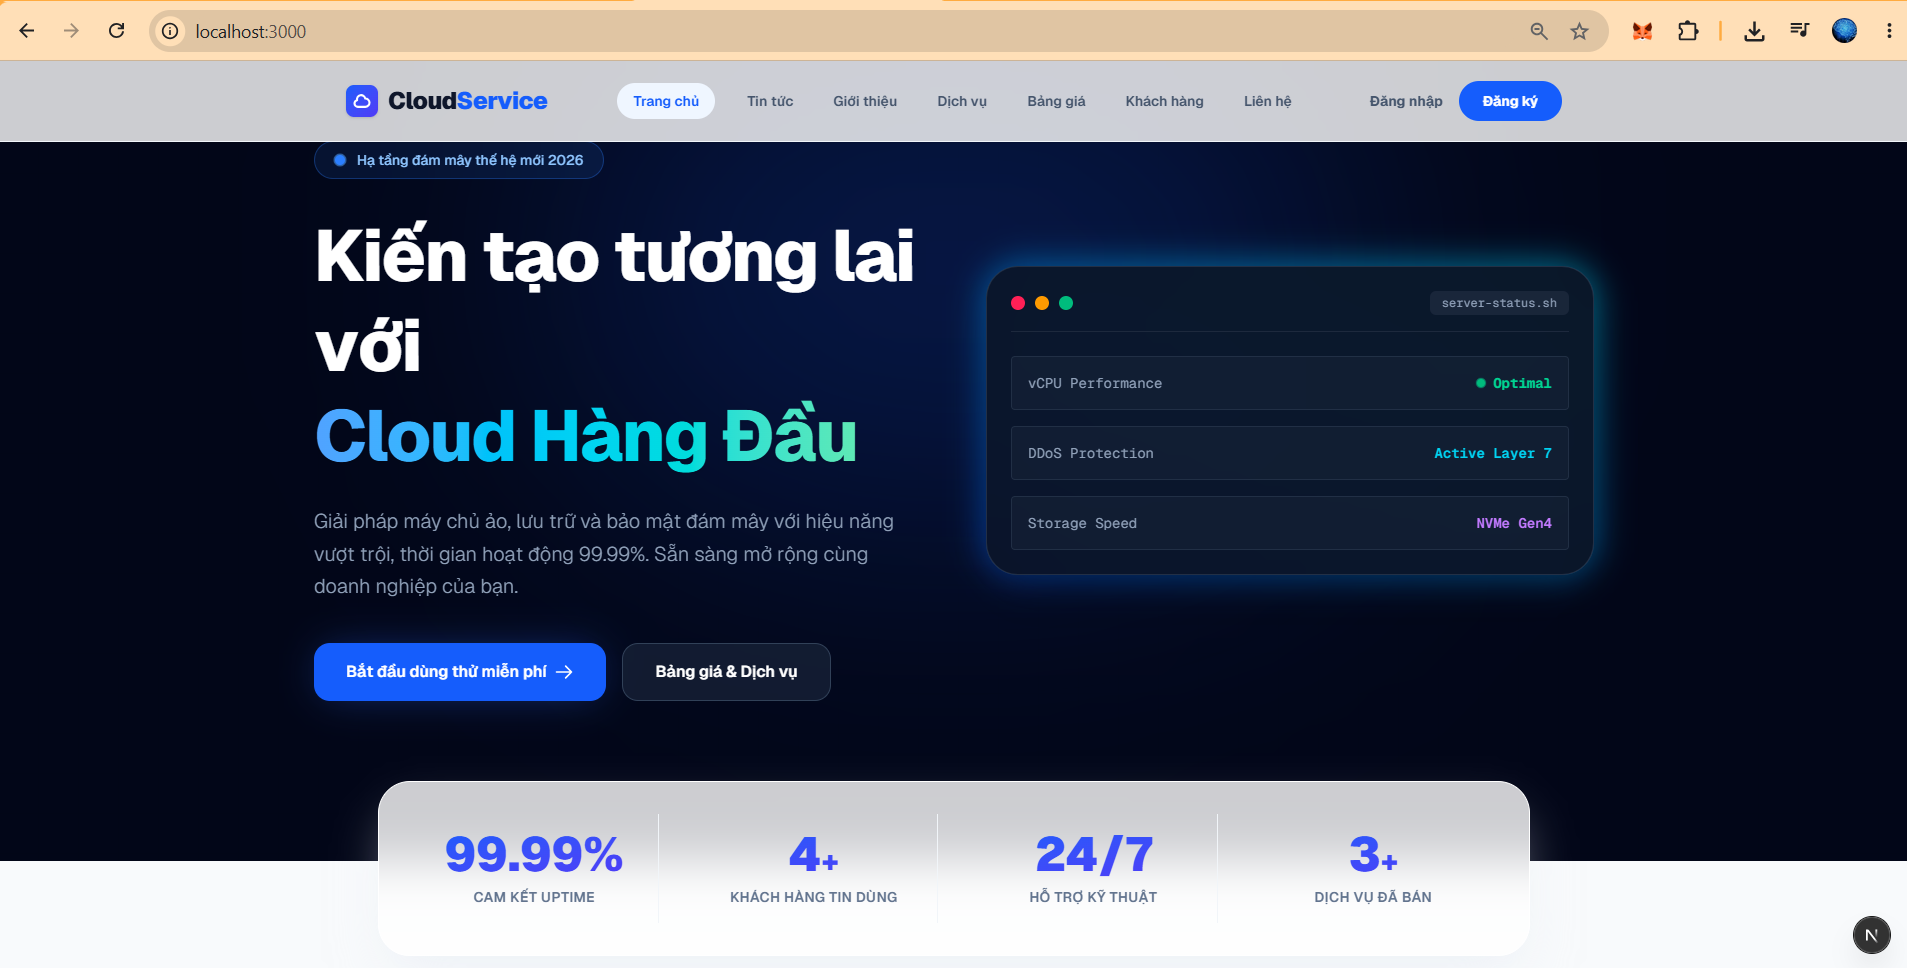
\includegraphics[width=0.9\textwidth]{images/landing_home.png}
    \caption{Giao diện trang chủ (Landing Page)}
    \label{fig:landing_home}
\end{figure}

% TODO: Chèn ảnh giao diện trang Bảng giá. Hãy lưu file ảnh tên là 'landing_pricing.png' vào thư mục 'images'
\begin{figure}[htbp]
    \centering
    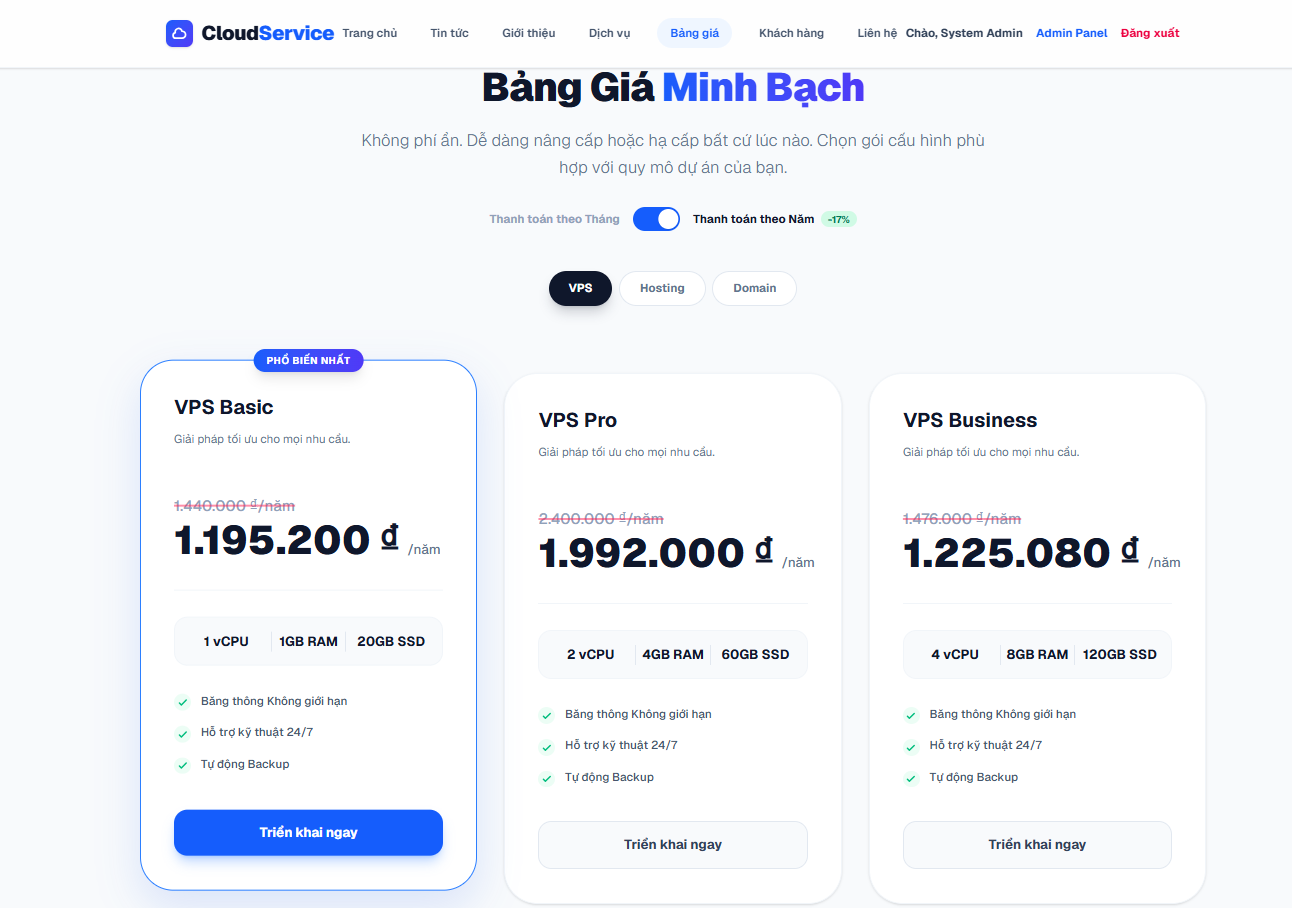
\includegraphics[width=0.9\textwidth]{images/landing_pricing.png}
    \caption{Giao diện trang Bảng giá -- Chuyển đổi Tháng/Năm và hiển thị mã QR}
    \label{fig:landing_pricing}
\end{figure}

\subsection{Giao diện Quản trị (Admin Dashboard)}
Sau khi xác thực thành công qua JWT tại trang \texttt{/login}, hệ thống dựa vào Role của người dùng để điều hướng đến Admin Dashboard. Giao diện quản trị bao gồm sidebar navigation cố định bên trái và khu vực nội dung chính bên phải.

Các trang Admin chính bao gồm:
\begin{itemize}
    \item \textbf{Dashboard:} Hiển thị thống kê tổng quan (tổng đơn hàng, doanh thu, số bài viết) qua các thẻ card và biểu đồ doanh thu theo tháng, dữ liệu lấy từ API \texttt{/admin/stats/summary} và \texttt{/admin/stats/revenue-chart}.
    \item \textbf{Quản lý Tin tức:} Hỗ trợ CRUD đầy đủ (Thêm/Sửa/Xóa bài viết) qua modal form, dữ liệu đồng bộ real-time với Backend.
    \item \textbf{Quản lý Đơn hàng:} Hiển thị danh sách đơn hàng, cho phép thay đổi trạng thái (Pending $\rightarrow$ Processing $\rightarrow$ Completed/Rejected) và xuất ra file Excel.
    \item \textbf{Quản lý Khuyến mãi:} Tạo và xóa chương trình khuyến mãi (mã code, phần trăm giảm, thời hạn).
    \item \textbf{Audit Logs:} Xem lịch sử hành động của hệ thống (ai đăng nhập, từ IP nào, lúc mấy giờ).
\end{itemize}

% TODO: Chèn ảnh giao diện Admin Dashboard. Hãy lưu file ảnh tên là 'dashboard_admin.png' vào thư mục 'images'
\begin{figure}[htbp]
    \centering
    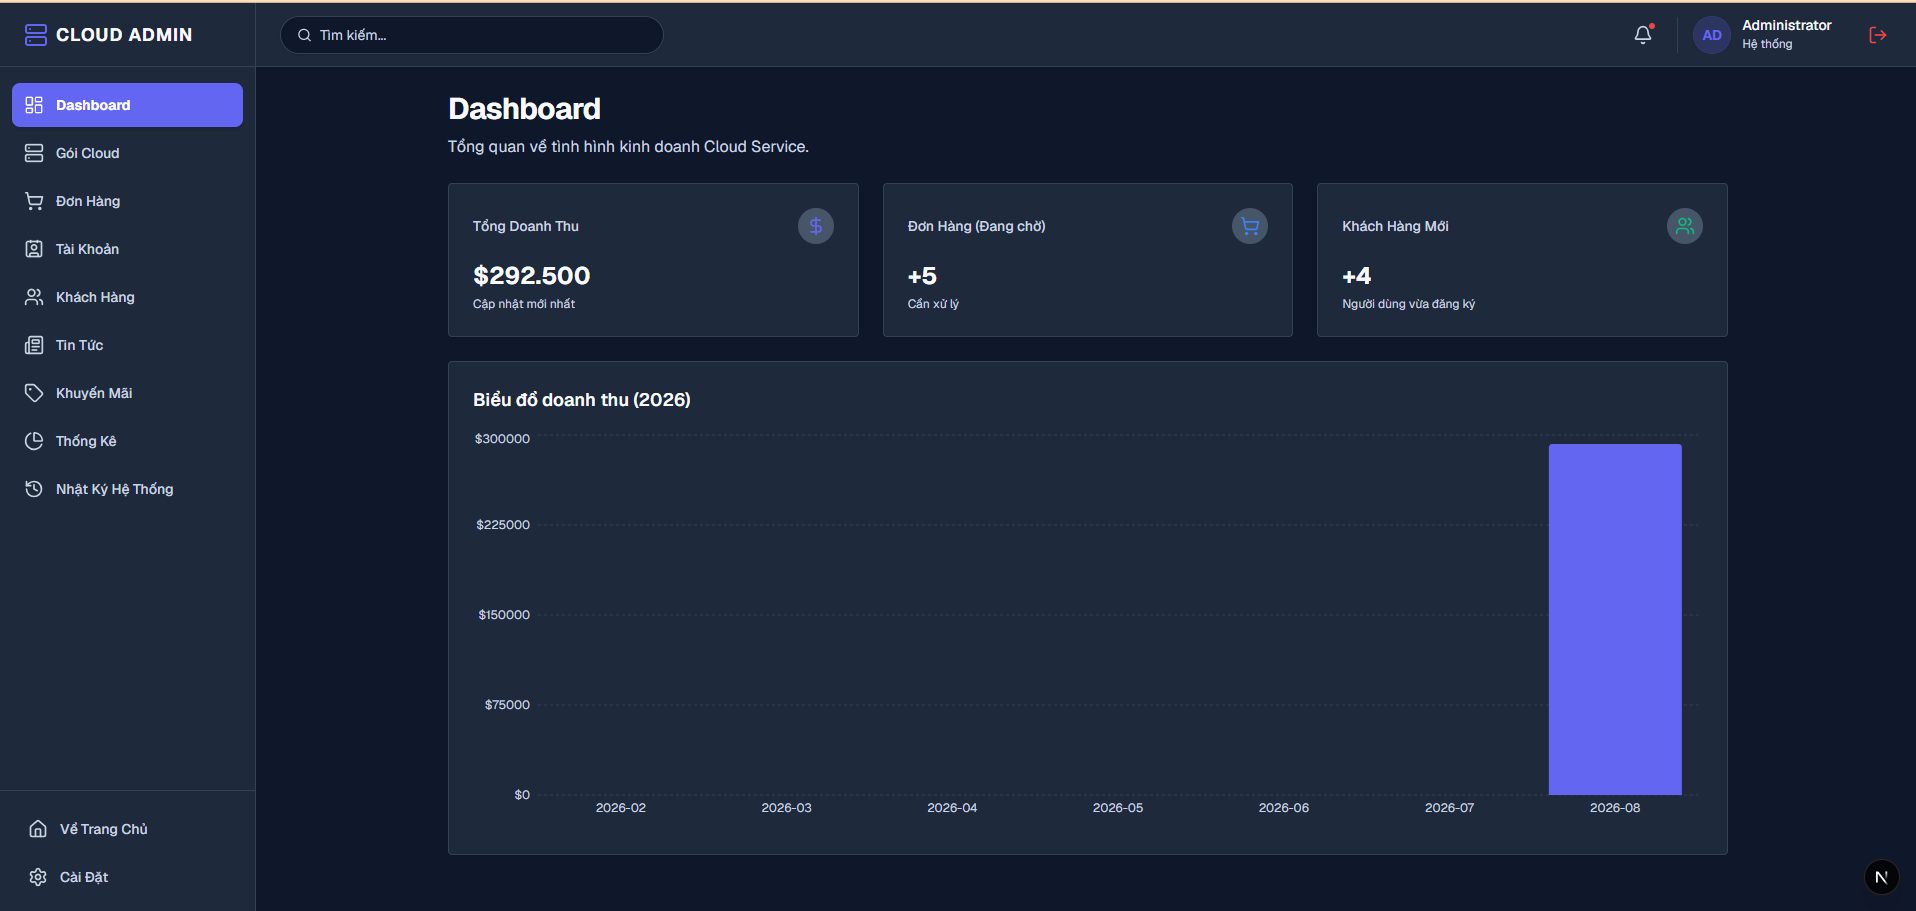
\includegraphics[width=0.9\textwidth]{images/dashboard_admin.png}
    \caption{Giao diện Bảng điều khiển Quản trị viên (Admin Dashboard)}
    \label{fig:dashboard_admin}
\end{figure}

\section{Kiểm thử đơn vị (Unit Testing)}
Kiểm thử phần mềm là một khâu không thể thiếu để đảm bảo độ tin cậy của sản phẩm. Dự án đã viết mã kiểm thử tự động sử dụng framework \textbf{xUnit} và thư viện mock \textbf{Moq} trên .NET trong project riêng biệt \texttt{CloudService.UnitTests}.

\subsection{Tổng quan kết quả}
Tổng cộng \textbf{16 test cases} (vượt yêu cầu tối thiểu 15) đã được viết và chạy thành công, phân bổ theo 5 file test:

\begin{table}[htbp]
    \centering
    \caption{Chi tiết kết quả Unit Test}
    \label{tab:unit_tests}
    \begin{tabular}{|c|p{5cm}|c|p{5cm}|}
        \hline
        \textbf{STT} & \textbf{File Test} & \textbf{Số test} & \textbf{Đối tượng kiểm thử} \\
        \hline
        1 & \texttt{OrderServiceTests.cs} & 6 & Tạo đơn hàng, đổi trạng thái, validate input, lấy danh sách, xử lý lỗi \\
        \hline
        2 & \texttt{ServicePlanServiceTests.cs} & 5 & CRUD gói dịch vụ, tính giá theo chu kỳ, validate specs \\
        \hline
        3 & \texttt{AffiliateServiceTests.cs} & 2 & Tạo đơn đăng ký affiliate, đổi trạng thái \\
        \hline
        4 & \texttt{CategoryServiceTests.cs} & 2 & CRUD danh mục, kiểm tra trùng tên \\
        \hline
        5 & \texttt{NewsArticleServiceTests.cs} & 1 & Tạo bài viết mới, generate slug \\
        \hline
        \multicolumn{2}{|c|}{\textbf{Tổng cộng}} & \textbf{16} & Tất cả PASSED \\
        \hline
    \end{tabular}
\end{table}

\subsection{Phương pháp Mock}
Mỗi test case sử dụng thư viện \textbf{Moq} để tạo đối tượng giả lập (mock) cho các Repository và UnitOfWork, giúp cô lập logic nghiệp vụ tại tầng Application mà không cần kết nối đến cơ sở dữ liệu thực. Ví dụ trích code test:

\begin{verbatim}
[Fact]
public async Task CreateOrder_WithValidData_ReturnsSuccess()
{
    // Arrange - Tạo mock repository
    var mockRepo = new Mock<IOrderRequestRepository>();
    var mockUoW = new Mock<IUnitOfWork>();
    mockUoW.Setup(u => u.Orders).Returns(mockRepo.Object);

    var service = new OrderService(mockUoW.Object);
    var dto = new CreateOrderDto {
        CustomerName = "Nguyen Van A",
        Email = "test@email.com",
        ServiceName = "VPS Pro"
    };

    // Act - Gọi hàm cần test
    var result = await service.CreateAsync(dto);

    // Assert - Kiểm tra kết quả
    Assert.NotNull(result);
    mockUoW.Verify(u => u.CompleteAsync(), Times.Once);
}
\end{verbatim}

% TODO: Chèn ảnh kết quả chạy Test. Hãy lưu file ảnh tên là 'unit_test_result.png' vào thư mục 'images'
\begin{figure}[htbp]
    \centering
    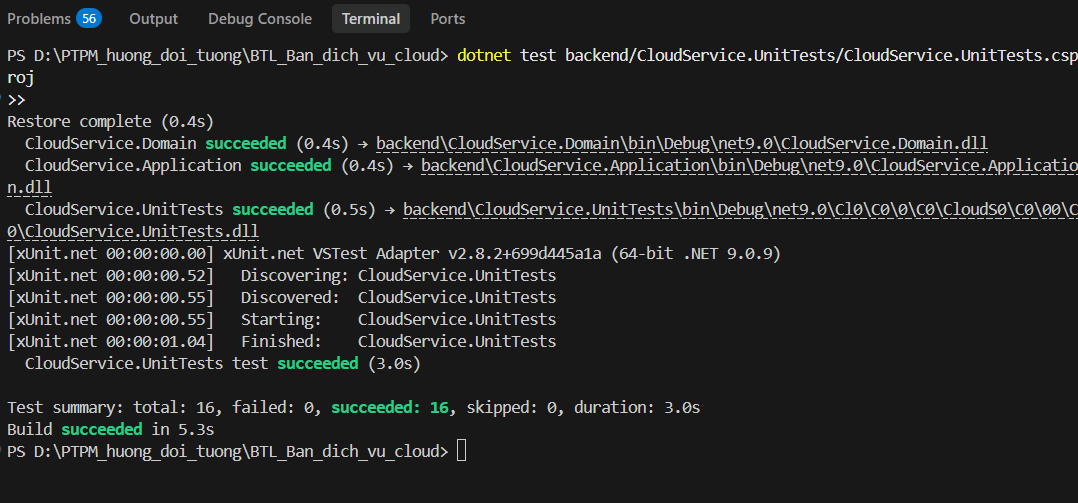
\includegraphics[width=0.8\textwidth]{images/unit_test_result.png}
    \caption{Kết quả chạy 16 Unit Test toàn bộ PASSED}
    \label{fig:unit_test_result}
\end{figure}

\section{Triển khai liên tục (CI/CD) và Docker}
Dự án áp dụng quy trình Phát triển phần mềm hiện đại, tuân thủ nguyên tắc ``Cộng tác chặt chẽ''. Mã nguồn được quản lý phiên bản qua Git trên GitHub.

\subsection{Luồng làm việc với GitHub Actions (CI)}
Mọi thao tác đẩy mã (Push) lên nhánh \texttt{develop} hoặc \texttt{main}, và mọi Pull Request đều kích hoạt pipeline GitHub Actions. Nội dung pipeline \texttt{.github/workflows/ci.yml}:

\begin{enumerate}
    \item \textbf{Checkout:} Kéo mã nguồn từ repository.
    \item \textbf{Setup .NET 9:} Cài đặt môi trường .NET SDK phiên bản 9.0.x.
    \item \textbf{Restore:} Khôi phục thư viện NuGet cho cả API và Unit Test project.
    \item \textbf{Build:} Biên dịch mã nguồn ở chế độ Release.
    \item \textbf{Test:} Chạy toàn bộ 16 Unit Tests. Nếu bất kỳ test nào thất bại, pipeline sẽ báo Failed và không cho phép merge PR.
\end{enumerate}

\subsection{Đóng gói ứng dụng với Docker}
Để giải quyết bài toán ``Chạy được trên máy tôi nhưng lỗi trên máy chủ'', toàn bộ hệ thống được cấu hình vào các Container riêng biệt:

\begin{itemize}
    \item \textbf{Dockerfile (Backend):} Multi-stage build: stage 1 (build) sử dụng image \texttt{dotnet/sdk:9.0} để biên dịch, stage 2 (runtime) sử dụng image \texttt{dotnet/aspnet:9.0} gọn nhẹ để chạy.
    \item \textbf{docker-compose.yml:} Định nghĩa 2 services:
    \begin{itemize}
        \item \texttt{sqldb}: SQL Server 2022 Express với dữ liệu lưu trên volume \texttt{sql\_data}.
        \item \texttt{backend}: API .NET 9 kết nối tới container \texttt{sqldb}, expose port 5000.
    \end{itemize}
\end{itemize}

Chỉ với một dòng lệnh duy nhất \texttt{docker compose up -d}, hệ thống đã được triển khai sẵn sàng trên mọi hệ điều hành hoặc máy chủ Cloud thực tế.

\subsection{Quy trình làm việc nhóm với Git}
Nhóm áp dụng mô hình \textbf{Feature Branch Workflow}:
\begin{enumerate}
    \item Mỗi tính năng được phát triển trên một nhánh riêng (ví dụ: \texttt{feature/admin-dashboard}).
    \item Khi hoàn thành, tạo Pull Request (PR) lên nhánh \texttt{develop}.
    \item Các thành viên khác review code và approve.
    \item CI pipeline tự động chạy build + test. Nếu PASSED, PR được phép merge.
    \item Nhánh \texttt{main} chỉ chứa code ổn định, sẵn sàng triển khai.
\end{enumerate}

\chapter{KẾT LUẬN VÀ HƯỚNG PHÁT TRIỂN}

\section{Đánh giá kết quả đạt được}
Kết thúc quá trình thực hiện đồ án môn học Phát triển phần mềm hướng đối tượng, nhóm đã hoàn thành các mục tiêu và yêu cầu từ giảng viên đề ra. Những kết quả nổi bật bao gồm:

\subsection{Khía cạnh Kỹ thuật}
\begin{itemize}
    \item Làm chủ và ứng dụng nhuần nhuyễn mô hình \textbf{Clean Architecture} đa tầng (4 project: Domain, Application, Infrastructure, WebApi).
    \item Khai thác hiệu quả các nguyên lý thiết kế \textbf{SOLID} và \textbf{Design Patterns} (Repository, Unit of Work, Middleware, Dependency Injection) để tạo ra một lõi phần mềm Backend linh hoạt, dễ nâng cấp.
    \item Xây dựng \textbf{37 RESTful API endpoints} hoàn chỉnh phục vụ cả trang công khai và trang quản trị.
    \item Phát triển \textbf{10 trang Landing Page} + \textbf{8 trang Admin Dashboard} với giao diện hiện đại sử dụng Next.js App Router và Tailwind CSS.
\end{itemize}

\subsection{Khía cạnh Nghiệp vụ}
\begin{itemize}
    \item Xây dựng thành công hệ thống website bán dịch vụ Cloud (VPS, Hosting, Domain) bao gồm toàn bộ luồng nghiệp vụ từ người dùng tra cứu, đăng ký đến phía admin phê duyệt và thống kê.
    \item Hệ thống xử lý tốt cơ chế bảo mật: xác thực JWT với AccessToken + RefreshToken, mã hóa mật khẩu bằng BCrypt, phân quyền theo Role (Admin, Editor).
    \item Tích hợp thành công các tính năng nâng cao: sinh mã QR cho gói dịch vụ, xuất báo cáo Excel, ghi nhật ký hệ thống (Audit Log).
\end{itemize}

\subsection{Khía cạnh Quy trình}
\begin{itemize}
    \item Vận dụng thực tế mô hình phát triển phần mềm thông qua việc chia nhỏ tính năng trên feature branch.
    \item Tích hợp luồng CI/CD (GitHub Actions) tự động build và chạy \textbf{16 Unit Tests} (vượt yêu cầu tối thiểu 15).
    \item Chuẩn hóa triển khai môi trường qua Docker: \texttt{Dockerfile} cho Backend và \texttt{docker-compose.yml} (API + SQL Server 2022).
\end{itemize}

Dự án không chỉ là minh chứng cho lượng kiến thức được lĩnh hội trong môn học mà còn giúp nhóm rèn luyện khả năng phối hợp làm việc thực tế, xử lý các luồng hợp nhất mã nguồn (Merge/Pull Request) trên Git.

\section{Bảng tổng hợp kết quả đối chiếu đề bài}
Bảng~\ref{tab:ket_qua} đối chiếu các tiêu chí chấm điểm từ đề bài với kết quả đạt được thực tế.

\begin{table}[htbp]
    \centering
    \caption{Đối chiếu kết quả đạt được với yêu cầu đề bài}
    \label{tab:ket_qua}
    \begin{tabular}{|p{7cm}|c|p{4.5cm}|}
        \hline
        \textbf{Tiêu chí} & \textbf{Điểm} & \textbf{Kết quả đạt được} \\
        \hline
        Clean Architecture + SOLID + Design Patterns & 20 & 4 tầng, 5 SOLID, 4 Patterns \\
        \hline
        Backend API đầy đủ, REST, ORM & 20 & 37 endpoints, EF Core, SQL Server \\
        \hline
        Frontend đầy đủ, responsive & 15 & 18+ trang, Responsive, SEO \\
        \hline
        Bảo mật: JWT + Role, Hash, QR & 10 & JWT + Refresh, BCrypt, QR Code \\
        \hline
        Unit Testing $\geq$ 15 tests & 10 & 16 tests (xUnit + Moq) \\
        \hline
        Git + CI/CD + Docker & 10 & GitHub Actions, Docker Compose \\
        \hline
        Báo cáo + Thuyết trình & 10 & Báo cáo LaTeX 5 chương \\
        \hline
        Vấn đáp & 5 & (Tại buổi demo) \\
        \hline
    \end{tabular}
\end{table}

\section{Phân công công việc}
Để có được một dự án phần mềm hoàn thiện, nhóm đã có sự phân bổ hợp lý nhiệm vụ, phát huy thế mạnh của từng thành viên:

\begin{table}[htbp]
    \centering
    \begin{tabular}{|c|p{3.5cm}|p{8.5cm}|}
        \hline
        \textbf{STT} & \textbf{Thành viên} & \textbf{Công việc phụ trách} \\
        \hline
        1 & [Nguyễn Trung Hậu] & \textbf{Team Lead / DevOps:} Phân tích yêu cầu, thiết kế CSDL (ERD). Xây dựng Backend tầng Domain và Application. Cấu hình Docker, CI/CD (GitHub Actions). Viết Unit Test (16 test cases). \\
        \hline
        2 & [Lương Quang Khải] & \textbf{Backend Developer:} Xây dựng RESTful API (14 Controllers, 37 endpoints). Triển khai xác thực JWT (Login, Refresh Token, Change Password), BCrypt hash, QR Code, Excel Export. Cấu hình Middleware (Audit, Exception). \\
        \hline
        3 & [Võ Phụng Tiên] & \textbf{Frontend Developer (Public):} Lập trình 10 trang Landing Page (Trang chủ, Giới thiệu, Dịch vụ, Bảng giá, Tin tức, Liên hệ, Đối tác, Khách hàng). Kết nối API cho form gửi đơn hàng và đăng ký affiliate. Responsive + Hamburger menu. \\
        \hline
        4 & [Phan Thành Vinh] & \textbf{Frontend Developer (Admin):} Lập trình 8 trang Admin Dashboard (Dashboard, Services, News, Orders, Affiliates, Promotions, Analytics, Audit Logs). Kết nối API CRUD. Viết báo cáo tổng kết đồ án. \\
        \hline
    \end{tabular}
    \caption{Bảng phân công công việc thực hiện dự án của nhóm}
    \label{tab:phan_cong}
\end{table}

\section{Hạn chế và Hướng phát triển trong tương lai}
Vì giới hạn thời gian thực hiện, hệ thống vẫn còn một số khía cạnh có thể tiếp tục nghiên cứu và mở rộng:
\begin{itemize}
    \item \textbf{Thanh toán điện tử (E-Payment):} Hiện tại tính năng đặt hàng dừng lại ở khâu ``Ghi nhận yêu cầu'', trong tương lai dự án có thể tích hợp API của các cổng thanh toán (như VNPay, MoMo) để tự động hóa khâu phê duyệt hóa đơn.
    \item \textbf{Tối ưu hóa hiệu năng (Caching):} Áp dụng bộ đệm (như Redis) ở tầng Backend để lưu trữ nhanh các truy vấn lặp lại (Bảng giá, Tin tức), giúp giảm tải cho cơ sở dữ liệu.
    \item \textbf{Quản lý Vi dịch vụ (Microservices):} Nếu quy mô ứng dụng mở rộng (số lượng khách hàng lớn), kiến trúc có thể được tách nhỏ thành các services độc lập (ví dụ: Identity Service, Order Service) để linh hoạt trong việc Scale-up.
    \item \textbf{Logging tập trung:} Tích hợp Serilog với Seq hoặc Elasticsearch để giám sát log tập trung, giúp debug và theo dõi hiệu suất hệ thống production.
    \item \textbf{Đăng ký tài khoản khách hàng:} Bổ sung luồng Register/Login riêng cho khách hàng (không phải Admin) để có thể theo dõi lịch sử đơn hàng cá nhân.
\end{itemize}

Đồ án đã tạo ra một nền móng công nghệ vững chắc. Với những hướng phát triển trên, sản phẩm hoàn toàn có tiềm năng để thương mại hóa trong môi trường công nghiệp điện toán đám mây.


% Tài liệu tham khảo
\cleardoublepage
\renewcommand{\bibname}{TÀI LIỆU THAM KHẢO}
\bibliographystyle{plain}
\bibliography{tai_lieu_tham_khao}

% Phụ lục
\chapter*{Phụ Lục}
\addcontentsline{toc}{chapter}{PHỤ LỤC}

\section*{Phụ lục A: Cấu trúc thư mục Backend}
\begin{verbatim}
backend/
|-- CloudService.Domain/           # Tang Domain (Core)
|   |-- Common/
|   |   \-- BaseEntity.cs          # Lop co so (Id, CreatedAt, UpdatedAt)
|   |-- Entities/
|   |   |-- ServiceCategory.cs     # Danh muc dich vu
|   |   |-- ServicePlan.cs         # Goi dich vu
|   |   |-- PlanPrice.cs           # Gia theo chu ky
|   |   |-- Promotion.cs           # Khuyen mai
|   |   |-- NewsArticle.cs         # Bai viet/Tin tuc
|   |   |-- OrderRequest.cs        # Yeu cau dat DV
|   |   |-- AffiliateApplication.cs # Dang ky doi tac
|   |   |-- AppUser.cs             # Tai khoan quan tri
|   |   \-- AuditLog.cs            # Nhat ky he thong
|   \-- Enums/
|       |-- UserRole.cs            # Admin, Editor
|       |-- OrderStatus.cs         # Pending, Processing...
|       \-- BillingCycle.cs        # Monthly, Yearly
|
|-- CloudService.Application/      # Tang Application
|   |-- Interfaces/                # 9 giao dien (Interface)
|   |-- Services/                  # 8 Service implementations
|   \-- DTOs/                      # Data Transfer Objects
|
|-- CloudService.Infrastructure/    # Tang Infrastructure
|   |-- Data/
|   |   |-- AppDbContext.cs        # EF Core DbContext
|   |   \-- Migrations/           # Database migrations
|   |-- Repositories/              # 7 Repository + UnitOfWork
|   \-- Services/
|       |-- JwtService.cs          # Sinh JWT Token
|       |-- PasswordHashService.cs # BCrypt hash
|       |-- QrCodeService.cs       # Sinh ma QR
|       |-- ExcelExportService.cs  # Xuat Excel
|       \-- AuthService.cs         # Xac thuc
|
|-- CloudService.WebApi/            # Tang Presentation
|   |-- Controllers/
|   |   |-- Public/                # 5 API cong khai
|   |   \-- Admin/                 # 9 API quan tri
|   |-- Middleware/
|   |   |-- ExceptionMiddleware.cs
|   |   \-- AuditMiddleware.cs
|   \-- Program.cs                 # DI + Pipeline config
|
|-- CloudService.UnitTests/         # Unit Test project
|   \-- Tests/                     # 5 file, 16 test cases
|
|-- Dockerfile                      # Multi-stage build
\-- docker-compose.yml              # API + SQL Server
\end{verbatim}

\section*{Phụ lục B: Cấu hình docker-compose.yml}
\begin{verbatim}
version: '3.8'
services:
  sqldb:
    image: mcr.microsoft.com/mssql/server:2022-latest
    container_name: cloudservice_db
    environment:
      - ACCEPT_EULA=Y
      - SA_PASSWORD=CloudService@2026!
      - MSSQL_PID=Express
    ports:
      - "1433:1433"
    volumes:
      - sql_data:/var/opt/mssql

  backend:
    build:
      context: ./backend
      dockerfile: Dockerfile
    container_name: cloudservice_api
    depends_on:
      - sqldb
    ports:
      - "5000:80"
    environment:
      - ASPNETCORE_ENVIRONMENT=Development
      - ConnectionStrings__Default=Server=sqldb;
        Database=CloudServiceDb;User=sa;
        Password=CloudService@2026!;
        TrustServerCertificate=True

volumes:
  sql_data:
\end{verbatim}

\section*{Phụ lục C: Cấu hình GitHub Actions CI}
\begin{verbatim}
name: .NET Backend CI
on:
  push:
    branches: [ "develop", "main" ]
  pull_request:
    branches: [ "develop", "main" ]

jobs:
  build-and-test:
    runs-on: ubuntu-latest
    steps:
    - uses: actions/checkout@v4
    - uses: actions/setup-dotnet@v4
      with:
        dotnet-version: '9.0.x'
    - name: Restore API
      run: dotnet restore backend/CloudService.WebApi/
           CloudService.WebApi.csproj
    - name: Restore Unit Test
      run: dotnet restore backend/CloudService.UnitTests/
           CloudService.UnitTests.csproj
    - name: Build
      run: dotnet build backend/CloudService.WebApi/
           CloudService.WebApi.csproj --no-restore -c Release
    - name: Run 16 Unit Tests
      run: dotnet test backend/CloudService.UnitTests/
           CloudService.UnitTests.csproj --no-restore
\end{verbatim}

\section*{Phụ lục D: Tài khoản Demo}
\begin{table}[htbp]
    \centering
    \begin{tabular}{|l|l|l|}
        \hline
        \textbf{Vai trò} & \textbf{Email} & \textbf{Mật khẩu} \\
        \hline
        Admin & admin@cloudservice.vn & Admin@123 \\
        \hline
        Customer & ustomer@gmail.com & Customer@123 \\
        \hline
    \end{tabular}
    \caption{Tài khoản demo cho hệ thống}
\end{table}
\textbf{Lưu ý:} Mật khẩu đã được mã hóa BCrypt trước khi lưu vào Database. Đây chỉ là tài khoản demo phục vụ mục đích kiểm thử.

\section*{Phụ lục E: Mã nguồn dự án}
Toàn bộ mã nguồn của dự án (bao gồm Backend, Frontend, file Docker và LaTeX báo cáo) được lưu trữ và quản lý phiên bản công khai trên GitHub tại địa chỉ:
\begin{itemize}
    \item \textbf{Link Repository:} \url{https://github.com/TrungHauNguyen4/CloudService-BTL-Nhom7.git}
\end{itemize}


\end{document}
